% !TeX root = seminar-ebert-scherer.tex
% TODO: remove all comments

\chapter{Single Sign On bei Webanwendungen}
\chapterauthor{Daniel Ebert und Sebastian Scherer}

\section{Einleitung} \label{EB_Einleitung}

Durch das \textit{Single Sign-on (SSO)} muss sich ein Benutzer nur einmal unter Zuhilfenahme eines einzigen Authentifizierungsverfahrens identifizieren \cite{EB52}. Danach übernimmt der SSO-Mechanismus die Aufgabe, den Anwender zu authentifizieren und die erkannte Identität zu bestätigen \cite{EB52}. Dies hat den Vorteil, dass sich der Benutzer nur einmal identifizieren muss und seine Identität sicher an weitere Systeme weitergegeben werden kann, ohne dass sich dieser dort erneut anmelden muss. Dadurch hat der Benutzer Zugriff auf mehrere Systeme, wie z.B. Frontend Anwendungen oder Backend Services, bei dem die Ressourcen für die authentifizierten und autorisierten Benutzer beschränkt ist.

\subsection{Motivation}

% Gute Graphiken für den Vortrag: https://www.renovodata.com/blog/2019/01/17/single-sign-on

SSO ist vor allem in Webanwendungen hilfreich, da der Benutzer dort oft mit vielen verschiedenen Systemen interagieren muss \cite{EB34}. Ohne SSO müssten sich Benutzer bei jedem System individuell und erneut mit einem separaten Account einloggen \cite{EB34}. Somit müsste sich der Benutzer mehrere Passwörter merken und bei jedem System einen manuellen Anmeldemechanismus durchführen. Dies senkt die psychologische Akzeptanz der Benutzer für die Sicherheit, da heutige Anmeldeprozesse Multi-Faktor Authentifizierung verwenden, welche Zeit und Aufwand benötigen.

In der Praxis wird daher in vielen Fällen dasselbe Passwort für mehrere Systeme verwendet. Werden dennoch unterschiedliche Passwörter verwendet, dann sind diese oft einfach gehalten, damit man sich alle Passwörter merken kann. Aus sicherheitstechnischer Sicht ist das nicht gut. Einfache Passwörter könnten z.B. durch Brute-Force oder durch Dictionary Attacks gebrochen werden. Immer dasselbe Passwort zu verwenden ist ebenfalls kritisch. Hat eines der Systeme einen Data Leak, dann könnten Angreifer Zugriff auf alle Systeme mit demselben Passwort erhalten. Dafür könnte zwar auch ein Password Manager verwendet werden \cite{EB34}. Bei diesen hat man allerdings immer noch das Problem der \textit{Psychological Acceptability} der Benutzer, da sich diese bei jedem System erneut registrieren und einloggen müssen. Hier schafft SSO Abhilfe.

\subsection{Vorteile von SSO}

%es gibt mehr Vorteile und Nachteile - wenn Zeit hinzufügen: https://www.renovodata.com/blog/2019/01/17/single-sign-on

Neben den im letzten Absatz erläuterten Vorteil der \textit{Psychological Acceptability} im Hinblick auf die Benutzer hat SSO auch Vorteile für die Entwickler. Bei SSO müssen sich diese nur um ein System zur Authentifizierung kümmern \cite{EB34}. Weiter sorgt SSO für eine simplere Administration, da alle Benutzerdaten in einem System aufbewahrt werden \cite{EB34}. Außerdem sind die Benutzer eher dazu bereit, ein sichereres Passwort zu verwenden, wenn sie wissen, dass sie sich nur ein Passwort merken müssen.

\subsection{Nachteile von SSO}

SSO hat auch Nachteile. Zum Beispiel kann es schwierig sein, SSO in bereits existierende Systeme einzubauen \cite{EB34}. Um dem entgegenzuwirken bieten SSO Lösungen wie \textit{Keycloak} fertige Adapter für verschiedene Programmiersprachen und Systeme an, wie z.B. für ReactJS \cite[OpenID Connect]{EB26} \cite{EB36}. Außerdem könnte man durch das SSO System einen \textit{Single Point of Failure} haben. Jedoch kann dem entgegengewirkt werden, beispielsweise bietet Keycloak die Möglichkeit an, mehrere Keycloak Instanzen zu verwenden \cite{EB33}. Diese Instanzen können auf mehrere Server verteilt werden, um die Redundanz zu erhöhen.

\subsection{Abgrenzung} \label{EB_Abgrenzung}

Es gibt verschiedene Arten von SSO \cite{EB38}. Diese Arbeit konzentriert sich auf SSO für Webanwendungen. Dabei interagiert der Benutzer mit webbasierten Anwendungen und Services.

Bei SSO können verschiedene Protokolle wie \textit{OAuth 2.0}, \textit{OpenID Connect(OIDC)} oder \textit{SAML 2.0} eingesetzt werden. Die OAuth 2.0-Spezifikation definiert lediglich ein Delegationsprotokoll, das für die Übermittlung von Autorisierungsentscheidungen über ein Netzwerk von webfähigen Anwendungen und APIs nützlich ist, jedoch kein Authentifizierungsprotokoll. Durch Authentifizierung soll festgestellt werden, dass der Benutzer derjenige ist, für den er sich ausgibt. Mit anderen Worten ist Authentifizierung der Nachweis einer Behauptung, wie z.B. der Identität eines Benutzers im System. In der Regel beweist er das, indem er einer Anwendung eine Reihe von Anmeldedaten, wie Benutzername und Passwort, zur Verfügung stellt. \cite{SSEB_OAuth2inAction} \label{SSEB_OAuthForAuthentication}

OAuth 2.0 allein ist kein Mechanismus, um festzustellen, wer ein Benutzer ist oder wie er sich authentifiziert hat. Es sagt nur, dass ein Benutzer eine Anwendung delegiert hat, um in seinem Namen zu handeln. OAuth 2.0 stellt diese Delegation in Form eines Access Tokens zur Verfügung, das die Anwendung verwenden kann, um im Namen des Benutzers zu handeln. Das Access Token wird der API vorgelegt, dessen Anwendung weiß, wie sie überprüfen kann, ob das Access Token valide ist. \cite{SSEB_AuthorizationvsAuthentication}

Wird zum Beispiel in ein Hotel eingecheckt, erhält man eine Schlüsselkarte, mit der das zugewiesene Zimmer betreten werden kann. Die Schlüsselkarte sagt jedoch nichts darüber aus, wer der Hotelgast ist oder wie er sich an der Rezeption authentifiziert hat. Diese Karte kann für die Dauer des Aufenthalts für den Zugang zu dem Hotelzimmer verwendet werden. In ähnlicher Weise zeigt ein OAuth 2.0 Access Token nicht an, wer ein Benutzer ist. Der Token ist ein Schlüssel, welcher für den Zugriff auf Daten verwendet werden kann. \cite{SSEB_AuthorizationvsAuthentication}

OIDC ist ein Authentifizierungsprotokoll, das eine Erweiterung von OAuth 2.0 ist. OIDC ist ein vollwertiges Authentifizierungs- und Autorisierungsprotokoll. OIDC macht auch starken Gebrauch von den \textit{JSON Web Token (JWT)}-Standards. Diese Standards definieren ein JSON-Format für Identitäts-Token und Möglichkeiten, diese Daten auf kompakte und webfreundliche Weise digital zu signieren und zu verschlüsseln \cite{SSEB_RFC7519}. OIDC ist ein offener Standard, welcher von der OpenID Foundation im Februar 2014 veröffentlicht wurde \cite{EB4}.

In dieser Arbeit wird nur das OIDC Protokoll betrachtet, da dieses im Gegensatz zu SAML 2.0 speziell für Webanwendungen entwickelt worden ist und das modernere Protokoll ist \cite[OpenID Connect vs. SAML]{SSEB_keycloakDocs}. Außerdem ist OIDC besser für HTML5 / JavaScript-Anwendungen geeignet, da es auf der Client-Seite einfacher zu implementieren ist als SAML 2.0. Da Token im JSON-Format vorliegen, sind sie mittels JavaScript leichter zu verarbeiten \cite{SSEB_ssoProtocols}.

Es gibt verschiedene Implementierungen von SSO-Systemen. Eines der bekanntesten dieser Implementierung ist Keycloak. Keycloak ist Open Source und wird von Red Hat und einer Open Source Community entwickelt. Keycloak ist eine SSO-Lösung für Webanwendungen und RESTful Webdienste, die OpenID Connect unterstützt. Keycloak bietet anpassbare Benutzeroberflächen für Anmeldung, Registrierung, Administration und Kontoverwaltung. Ebenfalls kann die Authentifizierung auch an Identitätsanbieter von Drittanbietern wie Facebook und Google delegiert werden. \cite{SSEB_keycloakDocs}

Keycloak unterstützt sowohl OIDC als auch SAML 2.0 \cite{EB26}. Anwendungen, welche mit Keycloak interagieren, müssen eines der beiden Protokolle auswählen \cite{EB26}. Zusätzlich zu den SSO-Features implementiert Keycloak auch \textit{Role Based Access Control} \cite{EB3}. Dabei können einem Benutzer Rollen wie z.B. \textit{Kunde} oder \textit{Mitarbeiter} zugewiesen werden. Basierend auf der Rolle des Benutzers hat dieser Zugriff auf andere Ressourcen. Da der Fokus dieser Arbeit auf SSO liegt, wird Role Based Access Control in der Beispielanwendung verwendet, aber nicht erläutert.

\subsection{Vorgehen}

In der ersten Sektion der Arbeit wurde SSO vorgestellt zusammen mit zugehörigen Vor- und Nachteilen, sowie der Motivation und einer Abgrenzung der verschiedenen SSO Protokolle. Die darauffolgende Sektion beschreibt den Aufbau des SSO Protokolls OIDC. In der dritten Sektion werden die Schwachstellen und passenden Gegenmaßnahmen in einem Threat Model aufgeführt. In Sektion vier wird anhand einer Beispielwebanwendung SSO praktisch gezeigt. Zuletzt wird eine Zusammenfassung dieser Arbeit gegeben.


\section{Aufbau von OpenID Connect}

Das SSO-Protokoll OpenID Connect ersetzt mehrere manuelle Authentifizierungen bei verschiedenen Service Providern durch eine einzige manuelle Authentifizierung bei einem \textit{Identity Provider} \cite{SSEB_mladenov2016security}. Ein Identity Provider verwaltet die Identitäten mehrerer Endbenutzer, bietet spezifische Authentifizierungsmechanismen (z.B. Benutzername/Passwort oder 2-Faktoren) und erstellt Authentifizierungs-Token über authentifizierte Endbenutzer \cite{SSEB_mladenov2016security}. Das Token ist ein signiertes JSON-Web-Token. Diese Authentifizierungs-Token werden von einem \textit{Service Provider} verbraucht, der dem Endbenutzer in Abhängigkeit von der Token-Verifizierung den Zugang gewährt oder verweigert \cite{SSEB_mladenov2016security}.

Der Aufbau des OIDC Protokolls wird anhand von Keycloak in den folgenden Sektionen erklärt.

\subsection{Teilnehmer/Rollen}

Die Entitäten beim OIDC können wie folgt kategorisiert werden.

\subsubsection{Endbenutzer} \label{EB_End-Benutzer}

Endbenutzer, oder kurz Benutzer, sind Entitäten, die in der Lage sind, sich in das Keycloak System einzuloggen \cite[Core Concepts and Terms]{SSEB_keycloakDocs}. Der Endbenutzer ist der menschliche Teilnehmer. Informationen über den Benutzer und über die Authentifizierung des Benutzers können in \textit{Claims} gespeichert werden \cite[Terminology]{EB4}. Claims sind Key-Value Paare. Diese Keys und Values können beliebig gewählt werden. In OIDC gibt es allerdings Standardclaims wie zum Beispiel \texttt{sub, iss, email} und \texttt{address} mit einer vorgeschriebenen Beschreibung und teilweise mit einer vorgeschriebenen Funktion \cite[Standard Claims]{EB4}. Zum Beispiel ist \texttt{sub} eine Identifikationsnummer für den Benutzer vom Issuer (\texttt{iss}) \cite[Standard Claims]{EB4}. Ein Issuer weist eine \texttt{sub} nur einmal zu \cite[Claim Stability]{EB4}. Aus diesem Grund können andere Teilnehmer, wie z.B. der Client, mit der Kombination von \texttt{sub} und \texttt{iss} einen Benutzer eindeutig identifizieren \cite[Claim Stability]{EB4}. Im Beispiel in Sektion \ref{EB_Beispielwebanwendung} gibt es nur einen Issuer (eine Keycloak Instanz), wodurch Benutzer allein durch \texttt{sub} eindeutig identifiziert werden können. Für andere Claims wie z.B. \texttt{email} fordert das OpenID Connect Protokoll diese Einzigartigkeit nicht \cite[Claim Stability]{EB4}.

\subsubsection{Clients} \label{EB_Client}

Clients sind Entitäten, welche die Authentifizierung eines Benutzers anfordern können. Es gibt drei Arten von Clients \cite{SSEB_OAuth2inAction}.

Die erste Art von Client ruft andere Services im Namen des authentifizierten Benutzers auf \cite[Sec. 1.1]{SSEB_RFC6749} \cite[Managing Clients]{SSEB_keycloakDocs}. Das sind z.B. die Frontend- oder Browser-Anwendungen, welche vollständig im Webbrowser laufen und geschützte Ressourcen vom Backend Server anfordern. Obwohl der Code für die Anwendung von einem Web-Server bedient werden muss, wird der Code selbst nicht auf dem Server ausgeführt und der Web-Server behält nichts vom Laufzeitstatus der Anwendung bei \cite{SSEB_OAuth2inAction}. Stattdessen geschieht alles, was die Anwendung betrifft, auf dem Computer des Endbenutzers in dessen Speicher des Web-Browsers \cite{SSEB_OAuth2inAction}.

Bei der zweiten Art handelt es sich um Backend-Anwendungen, die auf einem entfernten Server ausgeführt werden und auf die über Web-Services oder ein Frontend zugegriffen wird \cite{SSEB_OAuth2inAction}. Die Konfiguration der Anwendung und ihr Laufzeitzustand werden auf dem Web-Server gehalten und die Browser-Verbindung wird in der Regel über ein Session-Cookie hergestellt. Diese Clients können Ressourcen bereitstellen, welche für die authentifizierten und autorisierten Benutzer beschränkt sind und können auch als geschützter \textit{Ressourcenserver} bezeichnet werden.

Die dritte Art sind native Anwendungen, die direkt auf dem Gerät des Endbenutzers laufen \cite{SSEB_OAuth2inAction}. Da sich diese Arbeit auf Web SSO fokussiert, werden diese nicht behandelt, und nur der Vollständigkeit halber erwähnt.

\subsubsection{OpenID Provider}

Der \textit{OpenID Provider} kann Benutzer authentifizieren und Claims der Benutzer speichern. Keycloak ist ein Beispiel für einen OpenID Provider. Ebenfalls stellen sie verschiedene Service-Endpunkte für Clients zur Verfügung \cite[Keycloak URI Endpoints]{SSEB_keycloakDocs}. Neben dem Endpunkt für die Authentifizierung eines Benutzers stellen OpenID Provider den \textit{UserInfo Endpoint} bereit \cite[UserInfo Endpoint]{EB4} \cite[Keycloak URI Endpoints]{SSEB_keycloakDocs}. Clients können dort mit einem Access Token des Benutzers alle oder einen bestimmten Teil der Claims des Benutzers abrufen \cite[UserInfo Endpoint]{EB4}. Über \textit{Scopes}, ein Feld des Access Tokens, wird festgelegt, welche Claims abrufen werden können \cite[Requesting Claims]{EB4}. Die verschiedenen Arten und der Aufbau der Tokens wird in der nächsten Sektion \ref{EB_Tokens} beschrieben.

Es gibt weitere Endpunkte des OpenID Providers, wie zum Beispiel Endpunkte um \textit{ID}, \textit{Access} und \textit{Refresh Tokens} anzufordern, um einen Benutzer auszuloggen oder um die Signatur eines Token zu validieren \cite[Keycloak URI Endpoints]{SSEB_keycloakDocs}. OpenID Provider können Benutzer selbst oder über einen externen Identity Provider wie Google, Github oder Stack Overflow authentifizieren \cite{EB7} \cite[Social Identity Providers]{SSEB_keycloakDocs}. Dementsprechend werden die Accountdaten lokal oder bei dem externen Identity Provider gespeichert.

Der OpenID Provider ist auch für das Verwalten der Clients verantwortlich. Zum Beispiel müssen sich Clients beim OpenID Provider registrieren, um am SSO teilzunehmen \cite[Client Registration]{EB26} \cite{EB57}. Zusätzlich kann der OpenID Provider festlegen, auf welche anderen Clients, z.B. Backend Services, und auf welche Informationen und Ressourcen, z.B. Claims, ein Client Zugriff hat \cite[Audience Support]{SSEB_keycloakDocs} \cite[ID Token]{EB4}. Das wird in der Beispielimplementierung in Sektion \ref{EB_Keycloak} näher erläutert.

\subsection{Tokens} \label{EB_Tokens}

Bei SSO mit OpenID Connect werden verschiedene Arten von Tokens eingesetzt. Bei OpenID Connect haben Tokens das JWT-Format \cite{SSEB_RFC7519}. Tokens werden vom OpenID Provider erstellt und mit der \textit{JSON Web Signature} vom OpenID Provider signiert \cite{EB5}. Tokens können optional über \textit{JSON Web Encryption} verschlüsselt werden \cite{EB5}. Da Tokens bei Webanwendungen üblicherweise über HTTPS übertragen werden und deshalb bereits verschlüsselt sind, ist eine erneute Verschlüsselung mit JSON Web Encryption dort nicht erforderlich. Der OpenID Provider kann verschiedene Arten von Token ausgeben mit jeweils verschiedenen Zielgruppen und Anwendungsfällen \cite[Token Endpoint]{EB4}.

Ein JWT setzt sich aus 3 Teilen zusammen. Im Header wird der Algorithmus genannt, welcher für die Signatur des Tokens verwendet wird \cite{EB5}. Der Signaturalgorithmus kann frei gewählt werden. Keycloak verwendet standardmäßig \textit{HMAC-SHA256}. Der Payload besteht aus einer Menge von sogenannten \textit{JWT Claims} \cite{EB5}. Ein JWT Claim ist, wie ein Claim bei OpenID Connect, ein Key-Value Paar. Im Payload können auch OpenID Connect Claims übertragen werden. Der dritte Teil enthält die Signatur der anderen zwei Teile. Die drei Teile sind jeweils \textit{Base64url} kodiert \cite{EB5}. In Abbildungen dieser Arbeit wird nur der dekodierte Payload gezeigt.

Im Nachfolgenden werden drei Arten von Tokens, ID Token, Access Token und Refresh Token, beschrieben. Diese drei Token werden nach einer erfolgreichen Authentifizierung eines Benutzers an den Client gesendet.

\subsubsection{ID Token}

Der ID Token enthält Claims über die Authentifizierung des Benutzers \cite[ID Token]{EB4}. Wenn vom Client gefordert, können optional weitere Claims mit Informationen über den Benutzer enthalten sein \cite[ID Token]{EB4}. Die folgende Auflistung zeigt ein Beispiel für ein ID Token.

\begin{lstlisting}[caption=Beispiel ID Token, captionpos=b]
{
	"exp": 1606058197,
	"iat": 1606057897,
	"auth_time": 1606057896,
	"jti": "c7e74c3e-dc1c-4790-bc47-4b787abe86dd",
	"iss": "http://keycloak/auth/realms/ExampleRealm",
	"aud": "frontend1",
	"sub": "85dd2d59-2ed9-407e-a745-b2f676095d4b",
	"typ": "ID",
	"azp": "frontend1",
	"nonce": "33f922fc-eacc-4ad0-81f7-580e865177df",
	"email_verified": false,
	"name": "Tom Smith",
	"preferred_username": "tom_smith",
	"given_name": "Tom",
	"family_name": "Smith",
	"email": "tomsmith@web.de"
}
\end{lstlisting}

Ein Beispiel Claim für die Authentifizierung des Benutzers ist \texttt{auth\_time}, welches den Zeitpunkt der Authentisierung in Unixzeit (Epoch) angibt \cite[ID Token]{EB4}. Der interessierte Leser findet eine Definition für die meisten hier gezeigten Claims unter \cite{EB7}. Einen Teil dieser Claims werden später noch näher erläutert, wie z.B. die \texttt{nonce} in Sektion \ref{EB_Authentifizierung_eines_Benutzers} und \texttt{aud} in Sektion \ref{EB_AccessToken}.

Der ID Token ist nur für den Client, welcher an der Authentifizierung des Benutzers beteiligt war, gedacht \cite{EB59}. Dieser Client kann durch den ID Token die Benutzererfahrung anpassen \cite[ID tokens]{EB8}, z.B. mit einer Willkommensnachricht mit dem Namen des Benutzers. Der ID Token sollte nicht für die Autorisierung verwendet werden, z.B. um geschützte Ressourcen von einem Backend Service abzurufen. Das ist die Aufgabe des im nächsten Abschnitt beschriebenen Access Tokens.

\subsubsection{Access Token} \label{EB_AccessToken}

Der Access Token wird für die Autorisierung des Benutzers verwendet \cite{SSEB_RFC6749}. Man kann ihn als Schlüssel für Ressourcen interpretieren. Er kann Informationen enthalten, die spezifizieren auf welche Ressourcen und Clients man mit dem Access Token Zugriff hat \cite[Audience Support]{SSEB_keycloakDocs}. In Web-SSO kann das Access Token z.B. als \texttt{Bearer} Token im HTTP \texttt{Authorization} Header an Backend Services enthalten sein \cite{SSEB_RFC6750}. Dies wird später in Sektion \ref{EB_Zugriff auf geschützte Ressourcen} näher erläutert.

Abgesehen von der ID des Benutzers, dem \texttt{sub} Claim, sollte der Access Token keine weiteren Informationen über den Benutzer oder die Authentifizierung des Benutzers enthalten \cite{EB7}. Falls ein Client trotzdem Benutzerinformationen benötigt, kann er die erlaubten Benutzer Claims mit dem Access Token bei dem UserInfo Endpunkt abfragen \cite[UserInfo Endpoint]{EB4}. Die nachfolgende Auflistung zeigt ein Beispiel für ein Access Token.

\begin{lstlisting}[caption=Beispiel Access Token, captionpos=b]
{
	"exp": 1606061497,
	"iat": 1606061197,
	"jti": "2239840b-86ff-41da-8e14-7acfbf05cb35",
	"iss": "http://keycloak/auth/realms/ExampleRealm",
	"aud": [
		"backendclientservice1",
		"backendclientservice2"
	],
	"sub": "85dd2d59-2ed9-407e-a745-b2f676095d4b",
	"typ": "Bearer",
	"azp": "frontend1",
	"nonce": "33f922fc-eacc-4ad0-81f7-580e865177df",
	"scope": "openid email profile"
}
\end{lstlisting}

Der \texttt{scope} Claim beschreibt sowohl welche Benutzer Claims über den UserInfo Endpunkt abgerufen werden können, als auch auf welche Ressourcen man mit dem Access Token Zugriff hat \cite[Requesting Claims]{EB4} \cite{EB7}. Ein Scope kann eine Menge von Claims beschreiben. Zum Beispiel hat man mit dem \texttt{profile} Scope Zugriff auf die Benutzer Claims \texttt{name}, \texttt{family\_name}, \texttt{preferred\_username} und Weitere beim UserInfo Endpunkt \cite[Requesting Claims]{EB4}. 

Der \texttt{aud} (Audience) Claim gibt an, für welche Clients das Access Token bestimmt ist \cite[ID Token]{EB4}. Erhält ein Client ein Access Token und befindet sich dieser Client nicht in der \texttt{aud} Liste des Access Tokens, dann sollten keine geschützten Ressourcen an den Sender zurückgeschickt werden \cite{EB59}.

\subsubsection{Refresh Token}

ID-, Access- und Refresh Token haben eine Verfallszeit \cite[Sec. 4.1.4]{SSEB_RFC7519} \cite[ID Token]{EB4}. Diese Verfallszeit ist im \texttt{exp} (Expiration Time) Claim als Unixzeit gespeichert \cite[Sec. 4.1.4]{SSEB_RFC7519}. Ist ein Token abgelaufen, dann ist er nicht mehr gültig \cite[Sec. 4.1.4]{SSEB_RFC7519}. Speziell das Access Token hat aus Sicherheitsgründen eine kurze Verfallszeit \cite{EB61}. In Keycloak ist standardmäßig eine Verfallszeit von 5 Minuten für den Access Token eingestellt.

Über den Refresh Token können neue ID-, Access-, und Refresh Tokens erstellt werden ohne, dass sich der Benutzer erneut authentifizieren muss. Der OpenID Provider bietet dafür einen Endpunkt an, bei dem ein Refresh Token durch gewünschte neue Tokens mit erneuerter Verfallszeit ausgetauscht werden kann \cite[Sec. 1.5]{SSEB_RFC6749}. Das Refresh Token kann auch verwendet werden, um einen Access Token mit weniger Rechten zu erhalten \cite{EB12}. Das Access Token mit weniger Rechten kann dann an potenziell weniger vertrauenswürdige Clients gesendet werden.

Das folgende Beispiel soll die Motivation für die Verfallszeit erläutern. Ein Benutzer kann sich sowohl über einen PC, als auch über einen Laptop mit demselben Account am System anmelden. Es gibt ein Refresh Token für den PC und einen für den Laptop. Falls der Laptop gestohlen werden sollte, dann kann das Refresh Token für den Laptop an einer Stelle, dem OpenID Provider, gesperrt werden. Ein Angreifer kann dann keine neuen Access Tokens mehr beim OpenID Provider anfordern. Der Benutzer kann weiterhin neue Access Tokens anfordern. Dadurch hat er über seinen PC weiterhin Zugriff auf seinen Account und kann weiter arbeiten. Ein Angreifer könnte allerdings trotzdem mit dem Access Token auf Ressourcen des Benutzers zugreifen, wenn dieser noch nicht abgelaufen ist. Aus diesem Grund muss bei der Wahl der Verfallszeit abgewogen werden. Je geringer die Verfallszeit ist, desto öfters müssen neue Tokens vom OpenID Provider angefordert werden. Dies erhöht die Last des OpenID Provider Servers. Je höher die Verfallszeit ist, desto mehr Zeit hat ein Angreifer, um möglicherweise auf geschützte Ressourcen des Benutzers zuzugreifen. Clients haben allerdings auch die Möglichkeit, Tokens beim OpenID Provider zu validieren. Dies wird in Sektion \ref{EB_Validieren des Access Tokens} näher erläutert.

\subsection{Protokoll-Flow} \label{EB_Flows}

Bei SSO kommen verschiedene Flows oder \textit{Authorization Grants} zum Einsatz. Wie in der Abgrenzung in Sektion \ref{EB_Abgrenzung} beschrieben, gibt es verschiedene Protokolle und auch mehrere Varianten innerhalb eines Protokolls. Deshalb werden in dieser Arbeit nicht alle Protokolle und Varianten erläutert. Diese Sektion soll kurz eine Übersicht über die wichtigsten Flows von OIDC bei Webanwendungen bieten, die auf den Authorization Grant von OAuth 2.0 aufbauen.

Der \textit{Authorization Code Flow} wird in der nächsten Sektion ausführlich beschrieben, da dieser am besten zum Use Case unseres praktischen Beispiels passt und der meist verwendete Flow ist. Als Alternative zum Authorization Code Flow bietet das OpenID Connect Protokoll den \textit{Implicit Flow} und den \textit{Hybrid Flow} an, um einen Benutzer zu authentifizieren. Diese zwei Alternativen haben beide eine bessere Performance \cite[Implicit and Hybrid Flow]{EB26} und eine kürzere Latenz als der Authorization Code Flow \cite[Code Flow]{EB20}. Trotzdem sollten beide, zumindest mit Keycloak, aus Sicherheitsgründen nicht verwendet werden, da bei beiden Access Tokens über den Browserverlauf geleakt werden können \cite{EB26} \cite[Implicit Flow]{SSEB_keycloakDocs}.

\subsection{Authorization Code Flow}

\subsubsection{Authentifizierung eines Benutzers} \label{EB_Authentifizierung_eines_Benutzers}

Der \textit{Authorization Code Flow} ist der Empfohlene, um einen Benutzer zu authentisieren oder um zu überprüfen, ob der Benutzer bereits authentisiert ist \cite[Authorization Code Flow]{SSEB_keycloakDocs}. 

Der Flow arbeitet mit \textit{Uniform Resource Identifier (URI)-Redirects} \cite{EB12}. Außerdem muss der Client eingehende HTTP-Anfragen vom OpenID Provider erhalten können \cite{EB12}. Für diese Bedingungen eignet sich z.B. ein Webbrowser. Die Abbildung \ref{fig:EB_AuthorizationCodeFlow} zeigt eine Übersicht des Authorization Code Flows. Der \textit{Authorization Server}, \textit{Token}- und \textit{UserInfo-Endpoint} werden vom OpenID Provider bereitgestellt \cite{EB12} \cite[Keycloak URI Endpoints]{SSEB_keycloakDocs}.

% https://www.keycloak.org/docs/latest/server_admin/index.html#authorization-code-flow
% https://openid.net/specs/openid-connect-core-1_0.html#CodeFlowAuth
% good step description: https://medium.com/@aminsaqi/a-survey-on-sso-authentication-protocols-security-and-performance-287dcb634bdd
% alternativ graphik, ist nicht besser: https://backstage.forgerock.com/docs/am/6/oidc1-guide/
\begin{figure}[!ht]
	\centering
	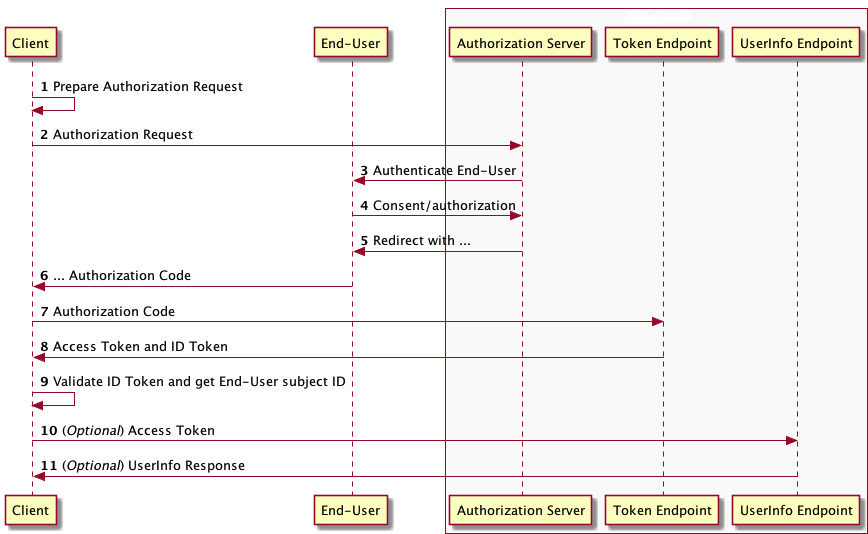
\includegraphics[width=1\textwidth]{Images/EbertScherer/AuthorizationCodeFlow.png}
	\caption{OIDC Authorization Code Flow Übersicht \cite{EB12}}
	\label{fig:EB_AuthorizationCodeFlow}
\end{figure} 

Als erstes wird der \textit{Authorization Request} vorbereitet. Diese Anfrage enthält mehrere Parameter im Query-String, einer davon ist die Identifikationsnummer des Clients \texttt{client\_id} \cite[Authentication Request]{EB4}. Diese ID wird bei der Registrierung des Clients beim OpenID Provider angegeben. Durch diese ID kann der OpenID Provider identifizieren, auf welche Scopes der Client Zugriff haben darf. Die Anfrage enthält auch eine Liste von gewünschten Scopes \texttt{scope}. Der \texttt{openid} Scope muss immer in der Liste der gewünschten Scopes angegeben werden \cite[Authentication Request]{EB4}. Dieser spezifiziert, dass es sich um eine OpenID Connect Anfrage handelt. Weiter muss eine \texttt{redirect\_uri} angegeben werden. Nach erfolgreicher oder fehlgeschlagener Authentifizierung wird der Browser des Benutzers zu dieser URI geleitet \cite[Authentication Request]{EB4}. Diese URI muss beim Registrieren des Clients mit angegeben werden. Optional kann in der Anfrage ein \texttt{state} hinzugefügt werden, dieser kann vor \textit{Cross-Site Request Forgery (CSRF)} schützen \cite[Authentication Request]{EB4}. Ebenfalls optional kann eine \texttt{nonce} angegeben werden, welche vor Replay Angriffen schützen kann \cite[Authentication Request]{EB4}. \texttt{state} und \texttt{nonce} werden später in Schritt 6 und 8 näher betrachtet. Listing \ref{EBAuthorizationRequest} zeigt ein Beispiel für einen Authorization Request. Über den \texttt{response\_type=code} wird der Authorization Code Flow ausgewählt. Mit \texttt{response\_mode=fragment} wird festgelegt, dass später ein Code per URI Fragment übertragen wird \cite[JavaScript Adapter Reference]{EB26}. Letzteres wird später in Schritt 5 und 6 näher erläutert.

\begin{lstlisting}[caption=Beispiel Authorization Request, captionpos=b, label=EBAuthorizationRequest]
GET https://keycloak/auth/realms/Test/protocol/openid-connect/auth?
        client_id=frontend1
        &redirect_uri=https%3A%2F%2Ffrontend.com%2F
        &state=0909ff6a-53b2-4253-8690-aff72d2cfff1
        &response_mode=fragment
        &response_type=code
        &scope=openid%20profile
        &nonce=67bad316-d8c1-45d1-9559-2a1c4726ce91
\end{lstlisting}

Im zweiten Schritt wird die Anfrage aus Schritt 1 an den Authorization Server, also den OpenID Provider, gesendet. Bei dieser Anfrage handelt es sich um eine GET HTTP-Anfrage. Was bedeutet, dass der Benutzer nach Schritt 2 nicht auf der Website des Clients, sondern auf der Website des OpenID Provider ist. Dies ist im Hinblick auf die Sicherheit wichtig, da sich der Benutzer im dritten Schritt authentisieren muss und seine Anmeldeinformationen wie z.B. Benutzername und Passwort eingeben muss. Da dies nicht auf der Seite des Clients passiert, sind die Anmeldeinformationen des Benutzers vom Client abgeschirmt \cite[How Does Security Work]{SSEB_keycloakDocs}. Das bedeutet, dass der Client keine Informationen über die Anmeldeinformationen des Benutzers hat. Der Client erhält nur die Tokens.

OIDC schreibt nicht vor, mit welchen Methoden der OpenID Provider den Benutzer in Schritt 3 authentifiziert \cite[Authorization Server Authenticates End-User]{EB4}. Als sicherere Alternative zu Benutzername und Passwort könnte hier z.B. auch eine Multi-Faktor-Authentifizierung eingesetzt werden. Auch die Methode, wenn der Benutzer bereits authentifiziert ist, wird vom OIDC Protokoll nicht vorgeschrieben. Zum Beispiel implementiert Keycloak das über HTTP Cookies. Nach einer erfolgreichen Authentifizierung, wird ein ID Token als \texttt{KEYCLOAK\_IDENTITY} Cookie für Keycloaks Authorization Endpunkt gesetzt \cite{EB17}. Bei Anfragen an Keycloaks Authorization Endpunkt ist dieses Token automatisch enthalten. Der Flow für bereits authentifizierte Benutzer ist dann größtenteils gleich, wie der für nicht authentifizierte Benutzer. Allerdings wird der Benutzer dann in Schritt 3 durch das Token und nicht durch die Eingabe von z.B. Benutzername und Passwort authentifiziert.

Nach erfolgreicher Authentifizierung muss der OpenID Provider in Schritt 4 sicherstellen, dass der Client für den Zugriff auf die von ihm gewünschten Scopes berechtigt ist. Im Vorhinein kann der Administrator des OpenID Providers die erlaubten Scopes für jeden Client festlegen \cite{EB68}. Optional kann in diesem Schritt auch ein interaktiver Dialog mit dem Benutzer stattfinden \cite[Authorization Server Obtains End-User Consent]{EB4}. Dabei wird dem Benutzer die Liste der gewünschten Scopes angezeigt. Der Benutzer hat hier die Möglichkeit den Scopes zuzustimmen oder die Authentifizierung abzubrechen.

In Schritt 5 und 6 wird der Benutzer bzw. der Browser zur \texttt{redirect\_uri} umgeleitet. Diese URI ist im Authorization Request von Schritt 1 spezifiziert worden. Die URI enthält einen vom OpenID Provider erstellten Code im Query-String oder im URI Fragment. Dieser Code wird Authorization Code genannt und ist für den Client opak \cite{EB67}. Seine Struktur wird also nur vom OpenID Provider verstanden. Der Authorization Code enthält Informationen über die Authentifizierung der vorherigen Schritte. Dazu gehören z.B. welche Scopes im Access Token enthalten sein werden. Der Authorization Code hat eine kurze Verfallszeit \cite[Authorization Code Flow]{SSEB_keycloakDocs}. Im Folgenden wird eine beispielhafte Redirect URI gezeigt.

\begin{lstlisting}[caption=Beispiel Redirect URI, captionpos=b, label=EBBeispielRedirectURI]
https://frontend.com/#
        state=0909ff6a-53b2-4253-8690-aff72d2cfff1&
        code=50342949-85bb-47ba-84ab-ed890b088226.0d9f3aa9-9e37-4c
        b7-a589-06972b3cf410.ef40a086-7a64-4b49-b3f0-11dc5cf92a68
\end{lstlisting}

Durch das im Authorization Request aus Schritt 1 angegebene \texttt{response\_mode=fragment} werden die Informationen über das URI Fragment übermittelt \cite[JavaScript Adapter Reference]{EB26}. Der in der Redirect URI zurückgegebene \texttt{state} muss derselbe sein wie in dem vorigen Authorization Request \cite[End-User Grants Authorization]{EB20}. Das verhindert CSRF, was später in der Sektion \ref{SSEB_Cross-Site-Request-Forgery} des Threat Models näher erläutert wird.

Der Authorization Code kann am Token Endpoint des OpenID Connect Providers zu einem ID, Access und optional einem Refresh Token ausgetauscht werden \cite[Token Endpoint]{EB4}. Dies wird in Schritt 7 und 8 per HTTP POST Anfrage durchgeführt \cite{EB20}. Um potenzielle Replay Angriffe zu verhindern, kann dieser Authorization Code nur einmal verwendet werden und hat eine sehr kurze Verfallszeit \cite[Authorization Code Flow]{SSEB_keycloakDocs}.

Durch die POST Anfrage werden die Tokens im HTTP Response Body zurückgegeben. Dadurch werden sie nicht dem Browser ausgesetzt \cite{EB22} und z.B. nicht im Browserverlauf gespeichert \cite[Implicit Flow]{SSEB_keycloakDocs}. Im Gegensatz dazu wurden Informationen wie z.B. der Authorization Code dem Browser ausgesetzt. Da der Access Token eine längere Verfallszeit hat und potentiell nicht widerrufen werden kann, sollte der Browser diesen aus Sicherheitsgründen nicht speichern \cite[Implicit Flow]{SSEB_keycloakDocs}.

In Schritt 8 muss das ID Token validiert werden. Dazu gehört zum Beispiel das Überprüfen der Signatur des Tokens \cite[ID Token Validation]{EB4}. Wird im Authorization Request in Schritt 1 eine \texttt{nonce} angegeben, dann muss der ID Token einen \texttt{nonce} Claim enthalten. Die \texttt{nonce} des Authorization Request muss mit der \texttt{nonce} des ID Tokens übereinstimmen. Außerdem muss die ID des Clients im \texttt{aud} Claim des ID Tokens enthalten sein, die \texttt{iss} muss die ID des OpenID Providers enthalten und der ID Token darf nicht bereits abgelaufen sein. Der \texttt{aud} und \texttt{iss} Claim wurden in Sektion \ref{EB_End-Benutzer} erläutert. Optional können weitere Validierungen stattfinden. Zum Beispiel kann ein Token abgelehnt werden, wenn die \texttt{auth\_time} zu weit in der Vergangenheit liegt. Diese und alle weiteren optionalen Validierungen werden in \cite[ID Token Validation]{EB4} aufgeführt.

Wie bereits in Sektion \ref{EB_AccessToken} erläutert, kann der ID Token nicht alle Benutzer Claims enthalten. Die durch den \texttt{scope} Claim des Access Tokens zugelassenen Benutzer Claims können abschließend optional über den UserInfo Endpunkt angefordert werden.

% kurz erwähnen dass sich clients dynamisch oder alternativ dass admin das macht in openid provider? kurz?

\subsubsection{Zugriff auf geschützte Ressourcen} \label{EB_Zugriff auf geschützte Ressourcen}

Der in dieser Sektion vorgestellte Prozess ermöglicht den Zugriff auf Ressourcen in anderen Clients, welche für die authentifizierten und autorisierten Benutzer beschränkt ist. Diese anderen Clients werden dabei, wie schon erwähnt, auch Ressourcen Server genannt. Dabei wird der Access Token dem Ressourcen Server übergeben. Der Standard schreibt nicht vor, wie dieses Übergeben des Access Tokens stattfinden soll \cite[Sec. 7]{SSEB_RFC6749}. Allerdings gibt der Standard an, dass das Access Token üblicherweise über den Authorization Header der HTTP Anfrage als sogenanntes Bearer Token übermittelt werden sollte \cite[Sec. 7]{SSEB_RFC6749}. 

Bearer Token bedeutet, dass jeder, der im Besitz des Tokens ist, das Token einsetzten kann \cite[Sec. 1.2]{SSEB_RFC6750}. Das bedeutet, dass der Ressourcen Server das Token an andere Clients senden kann, um von diesen Ressourcen abzurufen, z.B. in einer Microservice Architektur \cite{EB31}. Aus diesem Grund sollte man aus Sicherheitsgründen, vor allem wenn es möglicherweise nicht vertrauenswürdige Clients gibt, die erlaubten Scopes im Access Tokens analysieren und diese so weit wie möglich beschränken. Außerdem kann, wie in Sektion \ref{EB_AccessToken} beschrieben ist, über den Audience Claim im Access Token angegeben werden, für welche Clients das Access Token bestimmt ist. Der Ressourcen Server sollte validieren, dass seine Client ID im Audience Claim enthalten ist, bevor er angeforderte geschützte Daten zurücksendet \cite[Audience Support]{SSEB_keycloakDocs}.

\subsubsection{Validieren des Access Tokens} \label{EB_Validieren des Access Tokens}

Außer der im letzten Abschnitt erläuterten Validierung des Audience Claims, müssen weitere Informationen überprüft werden, bevor geschützte Daten vom Ressourcen Server herausgegeben werden. Dazu gehört die Überprüfung, ob das Token bereits abgelaufen ist \cite[Sec. 4.1.4]{SSEB_RFC7519}. Außerdem kann ein Ressourcen Server, basierend auf den erlaubten Scopes des Access Tokens, Entscheidungen treffen \cite[Sec. 3.3]{SSEB_RFC6749}. Zum Beispiel kann er die Herausgabe geschützter Daten aufgrund nicht vorhandener erlaubten Scopes verweigern \cite[Sec. 3.3]{SSEB_RFC6749}.

Zusätzlich muss das Access Token validiert werden. Grundsätzlich gibt es zwei verschiedene Varianten, wie das Access Token validiert werden kann. In dieser Sektion werden diese als Online und als Offline Variante bezeichnet.

\begin{figure}[!ht]
	\centering
	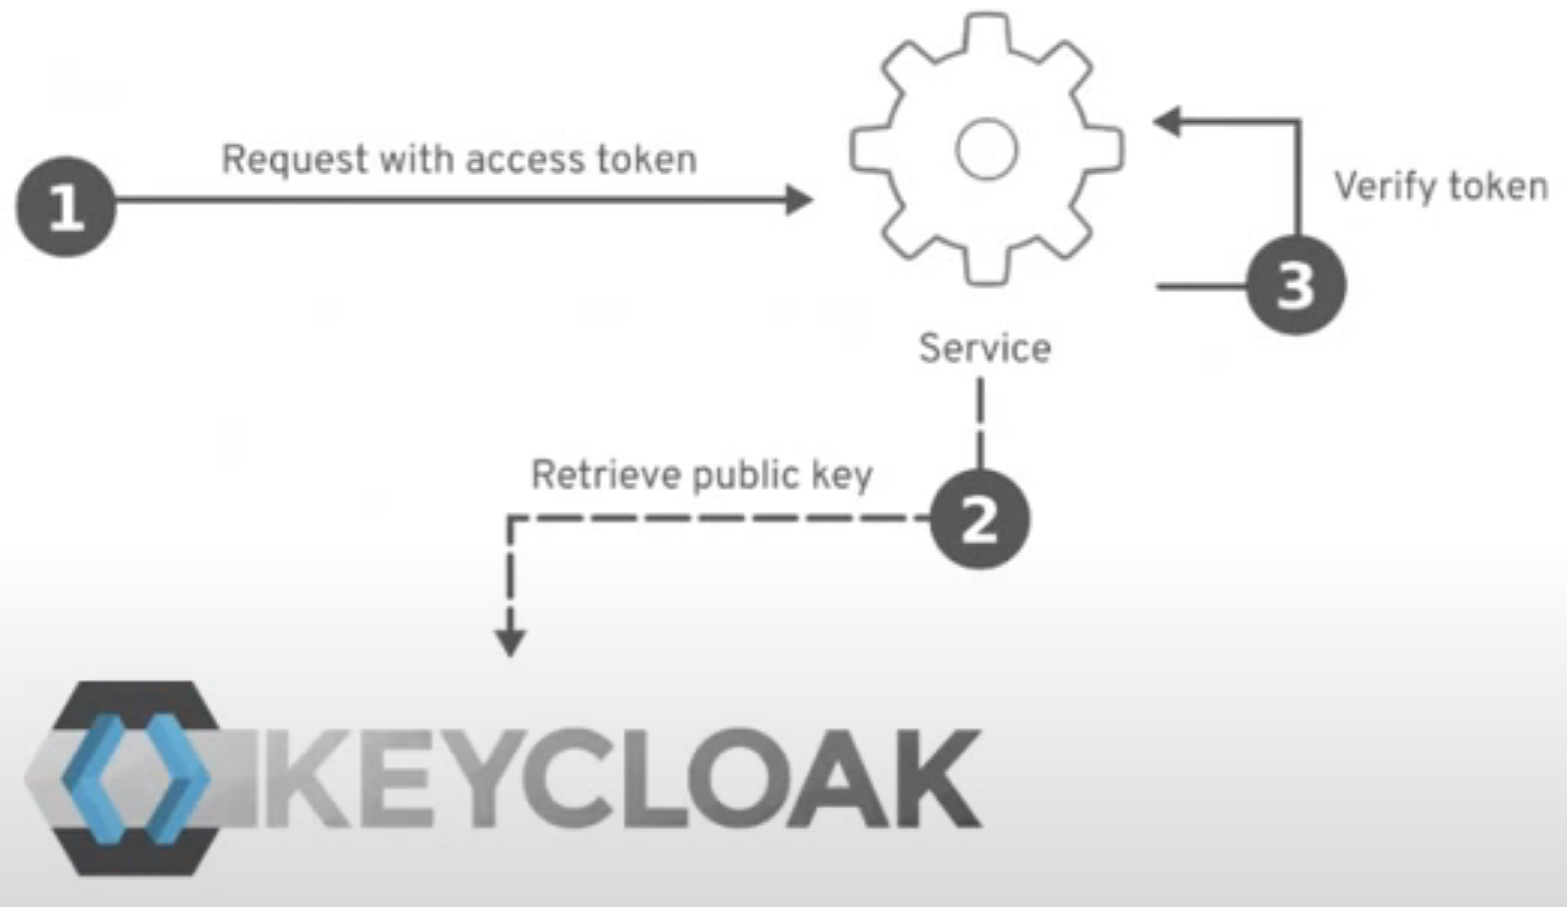
\includegraphics[width=.8\textwidth]{Images/EbertScherer/VerifyAccessTokenOffline.PNG}
	\caption{Access Token Verifizierung Offline Variante \cite{EB32}}
	\label{fig:EB_Access Token Verifizierung Offline Variante}
\end{figure}

In Abbildung \ref{fig:EB_Access Token Verifizierung Offline Variante} ist eine Übersicht der Offline Variante gezeigt. Dabei wird der Public Key, dessen Private Key vom OpenID Provider für die Signatur des Access Tokens verwendet wurde, vom OpenID Provider abgerufen. In der Abbildung ist Keycloak der OpenID Provider und der Client wird als Service bezeichnet. Der Client kann die Signatur des Access Tokens mit dem Public Key validieren.

Bei der Offline Variante wird der Public Key oft gecached \cite{EB32}. Das verringert die Latenz der Anfrage und die Auslastung des OpenID Provider Servers \cite{EB32}. Allerdings kann das Access Token dann nicht widerrufen und invalidiert werden. Aus diesem Grund haben Access Tokens im OpenID Connect Protokoll eine kurze Verfallszeit. Trotzdem bleibt dabei ein Zeitraum, in dem der erlaubte Zugriff eines Benutzers durch seine bereits existierenden Access Tokens nicht eingeschränkt werden kann. Um dieses Problem zu lösen, kann die Online Variante zur Validierung verwendet werden. % theorietisch könnte client bescheid gegeben werden > (ebert) richtig

\begin{figure}[!ht]
	\centering
	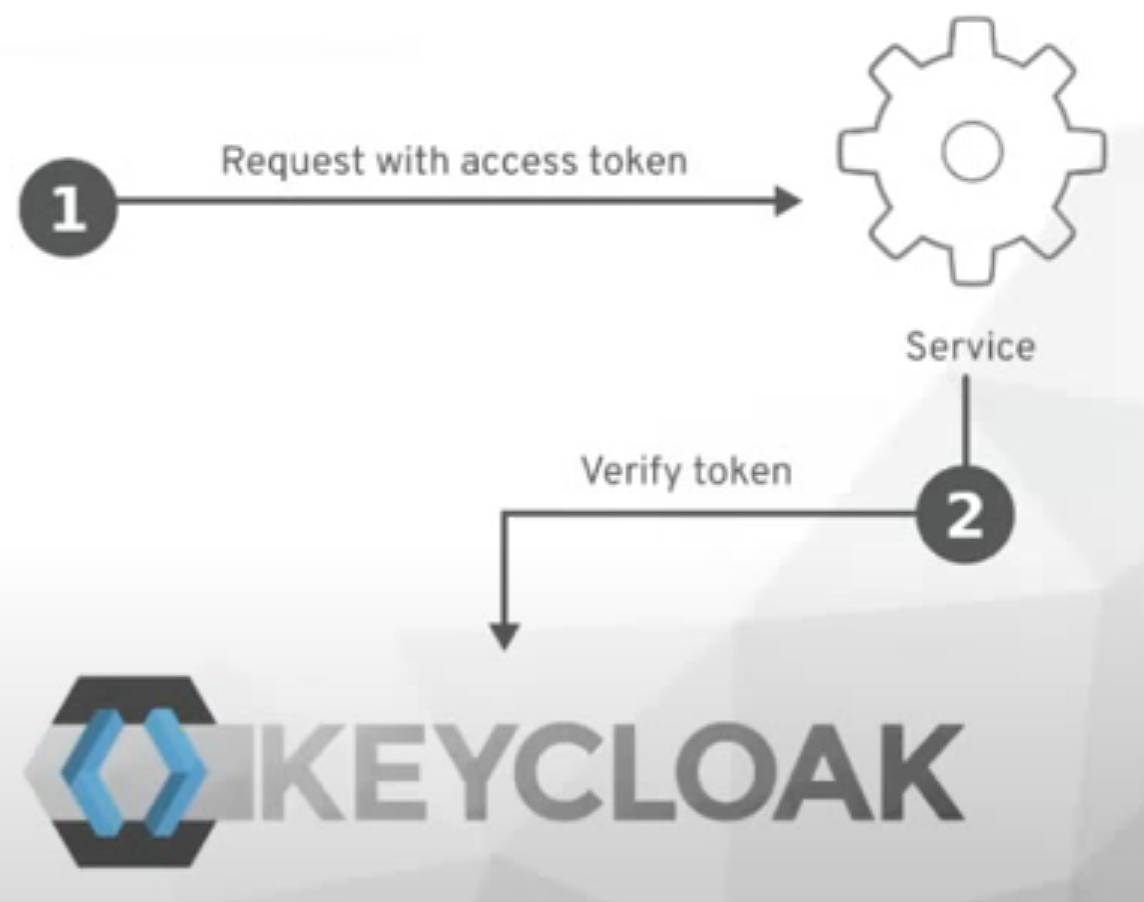
\includegraphics[width=.6\textwidth]{Images/EbertScherer/VerifyAccessTokenOnline.PNG}
	\caption{Access Token Verifizierung Online Variante \cite{EB32}}
	\label{fig:EB_Access Token Verifizierung Online Variante}
\end{figure}

Eine Übersicht der Online Variante wird in Abbildung \ref{fig:EB_Access Token Verifizierung Online Variante} gezeigt. Hier wird das Access Token bei jeder Anfrage an den OpenID Provider gesendet, um ihn dort zu verifizieren. Der OpenID Provider kann dann zusätzlich überprüfen, ob sich der Benutzer ausgeloggt hat, ob der Benutzer gesperrt wurde oder ob ein Administrator des OpenID Providers alle Access Tokens bis zu einem bestimmen Zeitpunkt gesperrt hat \cite{EB32}. Diese Maßnahmen greifen dann mit sofortiger Wirkung. Der Nachteil der Online Variante ist, dass jede Anfrage eine höhere Latenz hat und der OpenID Provider Server eine höhere Auslastung hat. Keycloak bietet für diese Variante einen separaten Endpunkt zur Validierung an. 

Den Nachteilen der Online Variante kann entgegengewirkt werden. Wie bereits in Sektion \ref{EB_Einleitung} erwähnt, bietet Keycloak die Möglichkeit an, mehrere Keycloak Instanzen zu verwenden \cite{EB33}. Dadurch kann die Last für den OpenID Provider auf mehrere Server verteilt werden. Darüber hinaus kann die Latenzzeit reduziert werden, indem z.B. der OpenID Provider Server und der Ressourcen Server im selben Rechenzentrum oder Rack betrieben werden.


\section{Threat Model} \label{SSEB_Threat Model}

In dieser Sektion werden mögliche Schwachstellen des OpenID Connect Protokolls erläutert. Weiter wird aufgeführt, wie diese mitigiert werden können. Eine Liste potenzieller Schwachstellen und was gegen sie getan werden muss, kann in dem von der IETF herausgegebenen Dokument \textit{OAuth 2.0 Threat Model and Security Considerations} \cite{SSEB_RFC6819} gefunden werden. Die am häufigsten vorkommenden und schwerwiegendsten Schwachstellen werden hier erörtert. \cite{SSEB_ssoProtocols}

Ein großer Teil der Sicherheit von OpenID Connect und OAuth 2.0 basiert auf der Annahme, dass Transport Layer Security (TLS) verwendet wird, um die Kommunikation zwischen den beteiligten Parteien zu sichern \cite{SSEB_mladenov2016security}. Es wird davon ausgegangen, dass die entsprechenden TLS-Kanäle sicher sind. Die Protokolle selbst sind frei von Kryptographie. Ebenfalls wird davon ausgegangen, dass der Endbenutzer nicht dazu verleitet werden kann vom Angreifer generierte TLS-Zertifikate als gültige Zertifikate für echte Clients zu akzeptieren \cite{SSEB_mladenov2016security}.

Obwohl OAuth 2.0 und OpenID Connect Sicherheitsprotokolle sind, garantiert ihre Verwendung allein noch keine Sicherheit. Sie müssen korrekt eingesetzt und verwaltet werden.

\subsection{OAuth 2.0 zur Authentifizierung}

Wie bereits erklärt, ist OAuth 2.0 ein fester Bestandteil für das Delegieren von Autorisierungen im Web und damit von SSO. Eine wichtige Einschränkung von OAuth 2.0 ist die Tatsache, dass es für die Autorisierung und nicht für die Authentifizierung konzipiert wurde \ref{SSEB_OAuthForAuthentication}. Die Verwendung von OAuth 2.0 zur Authentifizierung führt daher zu ernsthaften Schwachstellen.

Die Häufigkeit dieser Schwachstelle wurde in einer Feldstudie mit über 149 beliebten Anwendungen untersucht \cite{SSEB_chen2014oauth}. Das Ergebnis ist, dass 89 Anwendungen (59,7\%) OAuth 2.0 für Authentifizierung verwendet haben und damit anfällig sind \cite{SSEB_chen2014oauth}. Diese Studie verdeutlicht die Schwere dieses Basis-Threats.

Eine weitere Studie, die die Häufigkeit dieser Schwachstelle unterstreicht, wurde von Zhou et al. durchgeführt \cite{SSEB_184435}.

Daher muss OpenID Connect verwendet werden, welches auf OAuth 2.0 aufbaut, indem es Identitätsmanagement und Benutzerauthentifizierung bietet.

\subsection{Client Schwachstellen}

In dieser Sektion werden häufige Angriffen auf Clients präsentiert und praktische Möglichkeiten zur Verhinderung dieser Angriffe gezeigt.

Der Client hat Geheimnisse, wie Access und Refresh Tokens, für die er sicherstellen muss, dass diese an einem Ort aufbewahrt wird, der für Außenstehende nicht leicht zugänglich ist. Des Weiteren muss der Client darauf achten, dass diese Geheimnisse nicht versehentlich in Audit-Protokollen abgelegt werden, wo ein Dritter nach ihnen suchen könnte.

\subsubsection{Cross-Site-Request-Forgery} \label{SSEB_Cross-Site-Request-Forgery}

% Gute Erklärung: https://www.youtube.com/watch?v=_xrhWLqX1j0
% Der Client erzeugt das Token nicht der Server? - Ist sonst anders

Cross-Site-Request-Forgery (CSRF) tritt auf, wenn der Browser des Benutzers veranlasst wird eine unerwünschte Aktion durch eine Anfrage an eine Webanwendung auszuführen, auf der der Benutzer gerade per Cookie authentifiziert ist. Wenn ein Benutzer bei einer Anwendung angemeldet ist, kann ein Angreifer den Browser des Benutzers manipulieren, sodass er eine Anfrage stellt, an die das Cookie automatisch angehängt wird und die Anfrage als angemeldeter Benutzer ausgeführt wird. 

Um den Angriff durchzuführen, kann der Angreifer einen OAuth-Flow starten und einen Authorization Code vom Authorization Server erhalten. Der Angreifer veranlasst den Client des Opfers, den Authorization Code des Angreifers in einer bösartigen Anfrage zu verwenden, um den Code gegen einen Access Code einzutauschen. Der Ressourcenbesitzer hätte somit seine Client-Anwendung mit dem Autorisierungskontext des Angreifers verbunden. Dies hat katastrophale Folgen, wenn das OAuth-Protokoll zur Authentifizierung verwendet wird. \cite{SSEB_OAuth2inAction}

Die wirksamste Mitigation ist das Hinzufügen eines unvorhersehbaren Elements oder State-Tokens in jeder Anfrage. Der Zustandsparameter des Authorization Codes kann zur Vermeidung von CSRF verwendet werden. Dieser Parameter wird vom Client bei der Initialisierung der Session erstellt und an den Authorization Server gesendet, welcher diesen zurück sendet, um den Status zwischen jeder Anfrage und Antwort aufrechtzuerhalten. Versucht nun ein Angreifer dem Benutzer eine bösartige URL unterzuschieben, wird überprüft, ob die URL dieses State-Token enthält. Ist das State-Token nicht enthalten, verwirft der Client des Benutzers die URL des Angreifers und CSRF ist nicht mehr möglich. \cite{SSEB_OAuth2inAction}

Dieses State-Token wurde in Sektion \ref{EB_Authentifizierung_eines_Benutzers} bereits gezeigt. Das generierte State-Token kann in einem State-Cookie gespeichert werden.

Keycloak implementiert diesen Teil der Spezifikation vollständig, so dass alle Anmeldungen geschützt sind. Zum Beispiel ist die Keycloak Admin Console eine reine JavaScript/HTML5 Anwendung, die REST-Anfragen an die Keycloak Admin REST-API des Backend macht. Diese Anfragen erfordern alle eine Bearer-Token-Authentifizierung und werden über JavaScript-Ajax-Anfragen durchgeführt. CSRF ist hier nicht anwendbar. \cite{SSEB_keycloakDocs}

Der einzige Teil von Keycloak, der für CSRF anfällig ist, sind die Seiten zur Verwaltung der Benutzerkonten. Um dieses Problem zu entschärfen, setzt Keycloak ein Status-Cookie und bettet den Wert dieses Status-Cookies auch in versteckte Formularfelder oder Abfrageparameter in Aktionslinks ein. Dieser Abfrage- oder Formularparameter wird gegen das Status-Cookie geprüft, um zu verifizieren, dass die Anfrage durch den Benutzer erfolgt ist. \cite{SSEB_keycloakDocs}

\subsubsection{Registrierung der \texttt{redirect\_uri}}\label{Registrierung_redirect_uri}

Es ist äußerst wichtig, bei der Auswahl der registrierten \texttt{redirect\_uri} besonders darauf zu achten, dass die \texttt{redirect\_uri} so spezifisch wie möglich ist. Wenn die \texttt{redirect\_uri} nicht spezifisch ist, werden Token-Hijacking-Angriffe möglich. Wenn es möglich ist zu allgemeine \texttt{redirect\_uri} zu registrieren, ist es für einem Angreifer möglich, sich als ein Client auszugeben, welcher einen breiteren Zugriffsbereich hat \cite{SSEB_keycloakDocs}. Dies könnte zum Beispiel passieren, wenn zwei Clients die gleiche Domain besitzen \cite{SSEB_keycloakDocs}.

Der Hauptgrund dafür ist, dass Authorization Server unterschiedliche \texttt{redirect\_uri} Validierungsrichtlinien verwenden können. Die einzige zuverlässig sichere Validierungsmethode, die der Authorization Server anwenden sollte, ist die exakte Übereinstimmung \cite{SSEB_OAuth2inAction}. Alle anderen Lösungen, die auf Regular Expressions basieren oder Unterverzeichnisse des registrierten \texttt{redirect\_uri} zulassen, sind suboptimal und gefährlich \cite{SSEB_OAuth2inAction}.

\subsubsection{Diebstahl von Tokens}

Das Hauptziel eines Angreifers ist der Diebstahl eines Access Tokens. Mit dem Access Token könnte der Angreifer Operationen durchführen, für die er nicht autorisiert ist. 

Access Token werden an Ressourcenserver meist durch Übergabe des Inhaber-Tokens im Header (\texttt{Authorization: Bearer <Access Token>}) gesendet, jedoch definiert RFC 6750 weitere Methoden \cite{SSEB_RFC6750}. Einer davon ist der URI-Abfrageparameter, der es ermöglicht Access Tokens im URI über dem Abfrageparameter \texttt{access\_token} zu senden. Diese Methode kann zum Stehlen von Access Tokens verwendet werden. 

Wenn ein Angreifer in der Lage ist einen Link zu dieser Zielseite zu platzieren, dann wird im Referer-Header das Access Token offengelegt, da der Referrer die gesamte URL enthält  \cite{SSEB_OAuth2inAction}. Die Verwendung des Authorization Headers vermeidet diese Art von Problemen, da das Access Token nicht in der URL erscheint \cite{SSEB_OAuth2inAction}.

% \subsection{Client-Backend Schwachstellen}
% Eventuell Name zu Geschütze Ressourcen Schwachstellen und die andere section zu client allgemein - am besten ganz weg
% In dieser Sektionen sollen die Schwachstellen und Verteidigungen für Client-Backends, auch geschützter Ressourcenserver genannt, gezeigt werden. 
% Die geschützten Ressourcen des Client-Backends sind in mehrfacher Hinsicht verwundbar. Die erste entsteht durch Endpunktschwachstellen und die zweite durch Token Replays.

\subsubsection{XSS bei Endpunkten}

Wenn eine REST-API eingesetzt wird, bei der die Antwort von Benutzereingaben abhängt, ist das Risiko, auf eine XSS-Schwachstelle zu stoßen, hoch. Ein Endpunkt kann anfällig für Cross-Site-Scripting (XSS)-Angriffe sein, wenn der Ressourcenserver \texttt{access\_token} als URI-Parameter unterstützt. Dann kann der Angreifer eine URI fälschen, welche den XSS-Angriff in einem Inputwert enthält und dann Social Engineering einsetzen, um ein Opfer dazu zu bringen, diesem Link zu folgen. \cite{SSEB_OAuth2inAction}

Ist der Endpunkt für XSS anfällig ist, kann ein Angreifer eine bösartige URI fälschen, die auf die geschützte Ressource verweist. Sollte das Opfer diese Aufrufen, ist der Angriff abgeschlossen, wodurch die Ausführung des JavaScripts erzwungen wird \cite{SSEB_OAuth2inAction}. Der bösartige XSS-Code kann beispielsweise Daten extrahieren, um dem Angreifer die Möglichkeit zu geben, sich als authentifizierter Benutzer auszugeben. 

Die Output Sanitization ist der bevorzugte Ansatz zur Verteidigung gegen XSS. Des Weiteren kann der richtige \textit{Content-Type} in einer HTTP-Antwort zusätzlichen Schutz bieten. Wird beispielsweise der Content-Type \texttt{application/json} verwendet, wird die Antwort in JSON zurückgegeben und somit der XSS-Code nicht vom Browser ausgeführt. Ein weiterer nützlicher Response-Header, der von allen Browsern unterstützt wird, ist \texttt{X-Content-Type-Options: nosniff}. Dieser Sicherheitsheader verhindert, dass die Browser \textit{MIME Sniffing} für eine Antwort verwenden, die vom angegebenen Content-Type abweicht. Ebenso kann der Sicherheitsheader \texttt{X-XSS-Protection} gesetzt werden, der automatisch den XSS-Filter aktiviert, welcher in den meisten neueren Webbrowsern eingebaut ist. Ein weiterer nützlicher Response-Header gegen XSS ist \texttt{Content-Security-Policy (CSP)}, der in modernen Browsern deklariert, welche dynamischen Ressourcen über einen HTTP-Header geladen werden dürfen.

Die letzte Gegenmaßnahme, die ein Client implementieren kann, um jede Möglichkeit auszuschließen, dass ein bestimmter Endpunkt für XSS anfällig ist, ist das Übergeben von Access Tokens in den Anfrageparametern nicht zu unterstützen \cite{SSEB_OAuth2inAction}. XSS wäre auf dem Endpunkt theoretisch noch möglich, aber nicht ausnutzbar, da ein Angreifer keine Möglichkeit hat, eine URI zu fälschen, die auch das Access Token enthält\cite{SSEB_OAuth2inAction}. 

Daher muss das Access Token über den Authorization Header gesendet werden. In Keycloak wird die Authentifizierung über Authorization Header erzwungen \cite{SSEB_keycloakDocs}.

\subsubsection{Token Replays}

In einer vorherigen Sektion wurde gezeigt, wie es möglich ist, ein Access Token durch XSS zu stehlen. Selbst wenn die geschützte Ressource über HTTPS läuft, kann der Angreifer, sobald er das Access Token besitzt, auf die geschützte Ressource zugreifen. Aus diesem Grund ist es wichtig, ein Access Token zu haben, welches eine kurze Verfallszeit hat, um das Risiko des Token Replays zu minimieren. Selbst wenn es einem Angreifer gelingt, an ein Access Token zu gelangen, nimmt die Schwere des Angriffs ab, wenn dieses bereits abgelaufen ist oder kurz davorsteht. In der Sektion \ref{EB_Realms} wird gezeigt, wie die Verfallszeit des Access Tokens in Keycloak bestimmt werden kann.

OIDC und OAuth 2.0 sind frei von Kryptographie. Stattdessen verlassen sich die Protokolle vollständig auf das Vorhandensein von TLS über die verschiedenen Verbindungen hinweg. Aus diesem Grund gilt es die Verwendung von TLS im gesamten System so weit wie möglich durchzusetzen.

Dabei kann \textit{HTTP Strict Transport Security (HSTS)} helfen. HSTS erlaubt es zu definieren, dass Browser oder andere konforme User-Agents nur über sichere HTTPS-Verbindungen interagieren sollten und niemals über das unsichere HTTP-Protokoll. HSTS kann über den zusätzlichen HTTP-Header \texttt{Strict-Transport-Security} hinzugefügt werden. Jedes Mal, wenn versucht wird, den Endpunkt des Client-Backends mit dem Browser über HTTP zu erreichen, würde der Browser einen Redirect zu HTTPS durchführen. Dadurch wird jede unerwartete unverschlüsselte Kommunikation (wie z.B. Protokoll-Downgrade-Angriffe) vermieden. \cite{SSEB_OAuth2inAction}

Jedoch sollte nicht alleine auf HSTS vertraut werden, da es User-Agents gibt, die diesen Header nicht unterstützen und daher sollte in der Produktion nur HTTPS, beziehungsweise TLS, eingesetzt werden. In der Sektion \ref{EB_Realms} wird gezeigt, wie dies in Keycloak konfiguriert werden kann.

\subsection{Authorization Server Schwachstellen}

Der Authorization Server ist die komplexeste Komponente im SSO- und ODIC-System, und daher am schwersten zu sichern. In dieser Sektion werden dessen Schwachstellen präsentiert und gezeigt wie diese mitigiert werden müssen.

Für den Authorization Server gelten alle allgemeinen Sicherheitsmaßnahmen für den Einsatz sicherer Webserver. Besonders hervorzuheben sind Server-Logs, die Verwendung von TLS und eine sichere Hosting-Umgebung mit angemessenen Konto-Zugriffskontrollen.

\subsubsection{Session Hijacking}

In der Sektion \ref{EB_Authentifizierung_eines_Benutzers} wird erklärt, dass der Client einen Redirect-Schritt unternehmen muss, um an ein Access Token vom Authorization Server zu gelangen. Dieser Redirect veranlasst den Browser, eine Anfrage an den Client zu stellen, einschließlich des Authorization Codes.

Session Hijacking kann auftreten, wenn vertrauliche Clients verwendet werden. Bei diesert Art Clients verlässt der Authorization Code den Server und gelangt zum Benutzer. Dabei verbleibt der Authorization Code in der Browser-Historie.

Gelangt nun ein Angreifer auf den Rechner des Benutzers, kann sich dieser mit seinen eigenen Anmeldedaten anmelden, manipuliert jedoch den Redirect zum Client und injiziert den Authorization Code aus der Session des Benutzers, der im Browser-Verlauf gespeichert ist. Das Resultat ist, dass der Angreifer dann Zugriff auf die Ressource des ursprünglichen Benutzers hat.

Als Mitigation gegen diese Schwachstelle empfiehlt die OAuth 2.0 Spezifikation, dass Authorization Codes nur einmal vom Client verwendet werden dürfen \cite{SSEB_OAuthAuthorizationResponse}. Wenn ein Authorization Code mehr als einmal verwendet wird, muss der Authorization Server die Anfrage ablehnen und sollte alle Access Tokens zurücknehmen, die zuvor auf der Grundlage dieses Authorization Codes ausgegeben wurden \cite{SSEB_OAuthAuthorizationResponse}.

Diese Gegenmaßnahme wird durch Keycloak unterstützt. Ein Authorization Code kann nur einmal verwendet werden. Als zusätzliche Maßnahme ist die Verfallszeit für Authorization Codes sehr kurz - einige Sekunden, bei der der Benutzer seinen Authorization Code gegen ein Access Token eintauschen kann \cite[Sec. 19]{SSEB_keycloakDocs}.

\subsubsection{Redirection URI Manipulation}

Bei der Verwendung des Authorization Code Flows \ref{EB_Authentifizierung_eines_Benutzers} kann der Client eine Redirect-URI über den Parameter \texttt{redirect\_uri} angeben. Wenn ein Angreifer den Wert des Redirect-URIs manipulieren kann, kann er den Authorization Server veranlassen, den Benutzer einer Ressource zu einem URI unter der Kontrolle des Angreifers mit dem Authorization Code des Angreifers umzuleiten. \cite{SSEB_OAuthAuthorizationSecurityConsiderations}

Ein Angreifer kann einen Account bei einem Client erstellen und den Authorization Flow einleiten. Wenn der Benutzeraccount des Angreifers an den Authorization Server gesendet wird, um Zugriff zu gewähren, greift der Angreifer auf den vom Client bereitgestellten Authorization-URI zu und ersetzt den Redirect-URI des Clients durch einen URI unter der Kontrolle des Angreifers. Der Angreifer trickst dann den Benutzer einer Ressource aus, dem manipulierten Link zu folgen, um den Zugriff auf den Client zu autorisieren. \cite{SSEB_OAuthAuthorizationSecurityConsiderations}

Am Authorization Server wird dann dem Opfer über einen Client eine gültige Anfrage gestellt, welche dieser autorisiert. Das Opfer wird dann an einen Ressourcen-Endpunkt unter der Kontrolle des Angreifers mit dem Authorization Code umgeleitet. Der Angreifer schließt den Authorization Flow ab, indem er den Authorization Code an den Client, unter Verwendung der ursprünglichen Redirect-URI, sendet. Der Client tauscht den Authorization Code mit einem Access Token und verknüpft es mit dem Client-Account des Angreifers, welcher nun Zugang zu den geschützten Ressourcen erhalten kann. \cite{SSEB_OAuthAuthorizationSecurityConsiderations}

Um dieser Schwachstelle entgegenzuwirken, stellt der Authorization Server sicher, dass der Redirect-URI, der zum Erhalt des Authorization Codes verwendet wird, mit dem Redirect-URI identisch ist, welcher beim Austausch des Authorization Codes gegen ein Access Token bereitgestellt wird \cite{SSEB_OAuthAuthorizationSecurityConsiderations}\cite[Sec. 19]{SSEB_keycloakDocs}. Der Authorization Server muss von Clients verlangen, ihre Redirect-URIs zu registrieren \cite{SSEB_OAuthAuthorizationSecurityConsiderations}. Wenn in der Anfrage ein Redirect-URI angegeben wird, muss der Authorization Server diesen gegen den registrierten Wert der Redirect-URI validieren \cite[Sec. 19]{SSEB_keycloakDocs}.

\subsubsection{Open Redirector}

Der Authorization Server und der Client-Redirect-Endpunkt können so konfiguriert sein, sodass sie als \texttt{offene Redirector} funktionieren. Ein offener Redirector ist ein Endpunkt, der einen Parameter verwendet, um einen Benutzer ohne jegliche Validierung automatisch an den durch den Parameterwert angegebenen Ort umzuleiten. \cite{SSEB_OAuthAuthorizationSecurityConsiderations}

Offene Redirects können bei Phishing-Angriffen verwendet werden oder von einem Angreifer, um Benutzer dazu zu bringen, bösartige Seiten zu besuchen, indem die URI eines bekannten Ziels verwendet wird. \cite{SSEB_OAuthAuthorizationSecurityConsiderations}

Wenn der Authorization Server dem Client erlaubt, nur einen Teil der Redirect-URI zu registrieren, kann ein Angreifer darüber hinaus einen vom Client betriebenen offenen Redirector verwenden, um eine Redirect-URI zu konstruieren, die die Authorization Server-Validierung umgeht und Authorization Codes oder Access Tokens auf einen Endpunkt unter der Kontrolle des Angreifers sendet. \cite{SSEB_OAuthAuthorizationSecurityConsiderations}

Daher erfordert Keycloak, dass alle Clients mindestens ein Redirect-URI-Muster registrieren müssen. Jedes Mal, wenn ein Client Keycloak um eine Umleitung anfragt, überprüft Keycloak diesen Redirect-URI anhand der Liste der gültigen registrierten URI-Muster. Um offene Redirect-Angriffe abzuschwächen, müssen Clients möglichst spezifische URI-Muster verwenden. \cite[Sec. 19]{SSEB_keycloakDocs}

\subsection{Token Schwachstellen}

Die Schwachstellen der vorausgegangenen Sektionen hatten es meist zum Ziel ein Access Token oder einen Authorization Code zu erhalten. In dieser Sektion soll gezeigt werden welche Schwachstellen der Umgang mit den Tokens und Codes hat und wie diese Risiken minimiert werden können. 

% \subsubsection{Bearer Token}
% https://tools.ietf.org/html/rfc6750#section-5
% https://www.oauth.com/oauth2-servers/access-tokens/access-token-response/

Die OAuth 2.0 und OIDC-Spezifikationen verwenden Bearer-Token, sodass jeder, der im Besitz des Tokens ist, dieses verwenden kann, unabhängig davon wer er ist. Diese Bearer verwenden alle Klartextzeichen und benötigen daher TLS als Grundlage für die Sicherheit. \cite{SSEB_OAuthAuthorizationSecurityConsiderations}

In den Sektionen der vorherigen Sektionen wurde präsentiert, wie Access Tokens oder Authorization Tokens aus Clients gestohlen werden können. Bearer-Token für Clients sind transparent, damit keine kryptographischen Operationen durchgeführt werden müssen. Gelangt ein Angreifer an ein Token, ist er in der Lage, auf alle Ressourcen zuzugreifen, die in den Anwendungsbereich dieses speziellen Tokens fallen. Abgesehen vom Hijacking, welches in den vorherigen Sektionen bereits behandelt wurde, gibt es die folgenden Bedrohungen. Diese sind in vielen anderen tokenbasierten Protokollen ebenfalls zu finden:

\begin{itemize}
	\item \textit{Token Modification}: Ein Angreifer kann ein gefälschtes Token herstellen oder ein vorhandenes gültiges Token modifizieren, wodurch der Client-Ressourcenserver veranlasst wird, dem Client unangemessenen Zugriff zu gewähren. Beispielsweise kann ein Angreifer ein Token herstellen, um Zugang zu Informationen zu erhalten, die er zuvor nicht einsehen konnte. Alternativ könnte die Gültigkeit des Tokens selbst verlängert werden. \cite{SSEB_RFC6750}
	
	\item \textit{Token Replay}: Es wird ein altes, abgelaufenes Token wiederverwendet, um an valide Daten vom Ressourcenserver zu gelangen. Der Ressourcenserver sollte in diesem Fall einen Fehler zurückgeben. \cite{SSEB_RFC6750}
	
	\item \textit{Token Redirect}: Ein Angreifer verwendet ein Token, das für einen bestimmten Ressourcenserver generiert wurde, um Zugriff auf einen anderen Ressourcenserver zu erhalten Hierbei glaubt das Opfer fälschlicherweise, dass das Token für es gültig ist. \cite{SSEB_RFC6750}
	
	\item \textit{Token Disclosure}: Ein Token könnte sensible Informationen über das System enthalten und der Angreifer könnte an Informationen gelangen, für die er nicht berechtigt ist. \cite{SSEB_RFC6750}
\end{itemize}

Eine Gegenmaßnahme, die ein Client anwenden kann, besteht darin, den Umfang des Tokens auf das für seine Aufgaben erforderliche Minimum zu beschränken \cite{SSEB_OAuthAuthorizationSecurityConsiderations}. Dieser Ansatz der minimalen Privilegien schränkt ein, wofür das Token verwendet werden kann, wenn es erfasst wird. Um die Auswirkungen auf die Benutzererfahrung so gering wie möglich zu halten, kann ein Client während der Autorisierungsphase nach allen geeigneten Bereichen fragen und dann das Refresh-Token verwenden, um Access Token mit eingeschränktem Bereich zu erhalten, mit denen die Ressource direkt aufgerufen werden kann \cite{SSEB_OAuthAuthorizationSecurityConsiderations}. Diese Gegenmaßnahme wird insofern durch Keycloak unterstützt, dass in Umgebungen zwischen den einzelnen Services, unter denen das Vertrauen gering ist, der Empfängerkreis der Tokens limitiert werden kann \cite[Sec. 19]{SSEB_keycloakDocs}. Dies kann sowohl für die Scopes, als auch für die Audience konfiguriert werden \cite[Sec. 19]{SSEB_keycloakDocs}.

Um Angriffe zu minimieren, die sich aus den Injektionen in den Speicher ergeben, ist das Token im Transient Memory zu belassen. Browser löschen dann das Token, wenn der Browser vom Benutzer geschlossen wird.

Eine große Bandbreite von Bedrohungen kann durch den Schutz der Inhalte des Tokens abgemildert werden, durch Verwendung einer digitalen Signatur oder eines Message Authentication Codes (MAC) \cite{SSEB_RFC6750}. Der OAuth 2.0 Standard spezifiziert weder die Kodierung noch den Inhalt des Tokens, diese müssen selbst bestimmt werden. Der Schutz der Token-Integrität muss ausreichend sein, um eine Veränderung des Tokens zu verhindern  \cite{SSEB_RFC6750}. In Keycloak werden JWTs verwendet, welche signiert werden \cite[Sec. 19]{SSEB_keycloakDocs}. 

Um Token Redirects zu mitigieren, ist es wichtig, dass der Authorization Server die Identität der vorgesehenen Empfänger in das Token aufnimmt \cite{SSEB_RFC6750}\cite[Sec. 19]{SSEB_keycloakDocs}. In Keycloak wird durch den \texttt{sub}-Claim die Benutzer-ID mitaufgenommen.

Gegen Token Replay muss die Verfallszeit des Tokens gering sein \cite{SSEB_RFC6750}. Eine Möglichkeit, dies zu erreichen, besteht darin, ein Gültigkeitszeitfeld in den geschützten Teil des Tokens zu setzen. Je kürzer die Verfallszeit ist, desto geringer sind die Auswirkungen. Empfohlen wird eine Stunde oder weniger \cite{SSEB_RFC6750}. Da in Keycloak JWTs eingesetzt werden, haben die Tokens automatisch eine Ablaufzeit, welche durch den Keycloak Admin gesetzt werden kann. Des Weiteren können alle Tokens bei einer Kompromittierung widerrufen werden.


\section{Umsetzung von SSO innerhalb einer Beispielwebanwendung} \label{EB_Beispielwebanwendung}

%TODO Begriffe wie ressource server, clients, authorization server, access token mit einbauen
% am einfachsten ist es du packst die draw io datei zu deinen bildern ins repo, dann kann ich es auch bearbeiten - hat zeit
% (ebert) du hast recht, die begriffe müssen irgendwo mit rein. ich finde es schwierig die übersicht zu machen, weil wir das übersicht bild nicht zu detailliert machen sollten. ich habe die draw.io datei ins repo hochgeladen, vielleicht kannst du deine idee für die übersicht zeigen dann können wir nochmal darüber reden. vielleicht können wir auch unter dem übersicht bild einen absatz schreiben mit den begriffen, z.B. beim 'Zugriff auf geschützte Ressourcen' (rot) wird Access Token im Bearer Header mitgeschickt, blau verwendet Auth. Code Flow, green ist online token veri...
% (ebert) update: habe einen absatz zur übersicht geschrieben, inklusive der begriffe wie ressource server, clients - damit sollte die übersicht so passen
\begin{figure}[!ht]
	\centering
	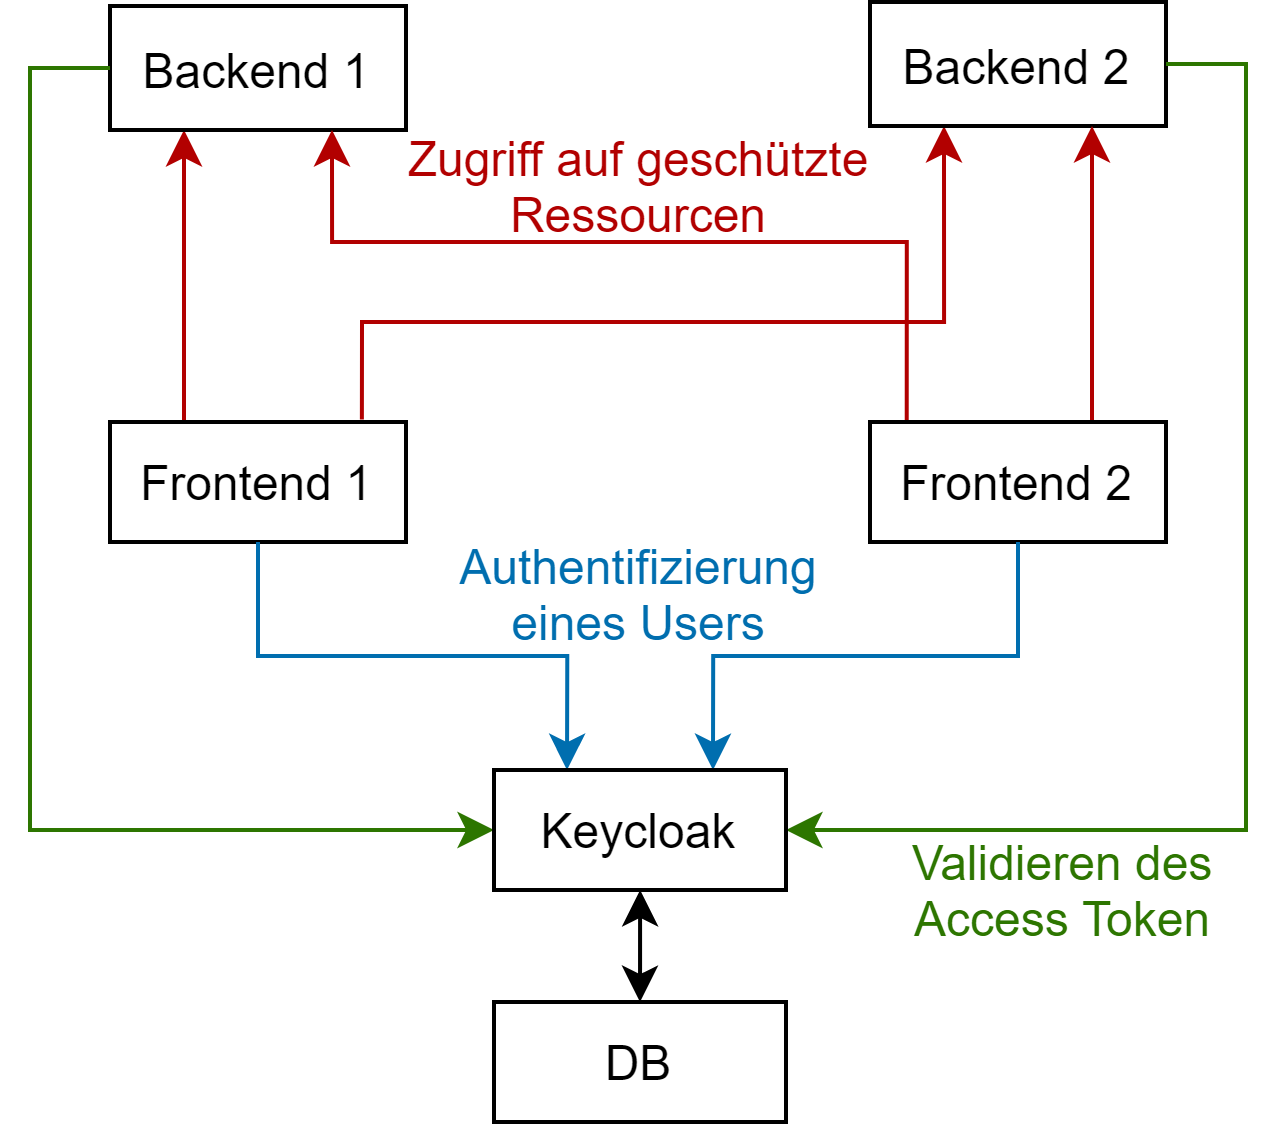
\includegraphics[width=.8\textwidth]{Images/EbertScherer/ArchitectureDiagram.png}
	\caption{Überblick der Beispielwebanwendung}
	\label{fig:EB_Beispielwebanwendung Überblick}
\end{figure}

Abbildung \ref{fig:EB_Beispielwebanwendung Überblick} zeigt einen Überblick über die Architektur und die Flows der implementierten Beispielwebanwendung. Jedes Rechteck stellt einen Microservice dar. Jeder Microservice läuft in einem separaten Docker Container. Pfeile stellen Flows bzw. Interaktionen zwischen den Services dar. Die Richtung der Pfeile gibt an, von welchem Service der Flow ausgeht. 

Die Namen und Funktionsweisen der Flows in Abbildung \ref{fig:EB_Beispielwebanwendung Überblick} korrespondieren mit den in Sektion \ref{EB_Flows} beschriebenen Flows. Frontend 1 und 2 sind die in Sektion \ref{EB_Client} beschriebenen Clients der ersten Art. Diese können mit dem Authorization Code Flow einen Benutzer authentifizieren. Dabei kommt Keycloak als OpenID Provider zum Einsatz. Keycloak speichert die Konfiguration der Clients und die Daten der Benutzer in einer Postgres Datenbank (DB) ab. Backend 1 und 2 nehmen am SSO Teil, stoßen selbst allerdings keinen Authentifizierungsflow an. In Sektion \ref{EB_Client} sind das die Ressourcenserver, also Clients der zweiten Art. Die Frontend Clients können HTTP Post Anfragen an die Backend Clients senden. In diesen Anfragen kann ein Access Token enthalten sein. Dieser Access Token wird von den Backend Clients beim OpenID Provider Keycloak validiert. Bei erfolgreicher Validierung senden die Backend Clients die Identifikationsnummer des authentifizierten Benutzers, den 'sub' Claim, mit HTTP Status Code 200 zurück.

Alle Docker Container werden mit Docker-Compose gestartet und konfiguriert. Docker-Compose ist ein Tool für Multi-Container-Anwendungen \cite{EB40}. Über Docker-Compose wird ein Netzwerk erstellt und konfiguriert. Dadurch können die Komponenten untereinander kommunizieren. Außerdem kann der Benutzer dadurch über den Browser mit den Komponenten kommunizieren. Über Docker-Compose wird ebenfalls ein persistenter Speicher für die Komponente DB (Datenbank) aufgesetzt und Umgebungsvariablen für die Anwendungen in den Containern gesetzt.

\begin{figure}[!ht]
	\centering
	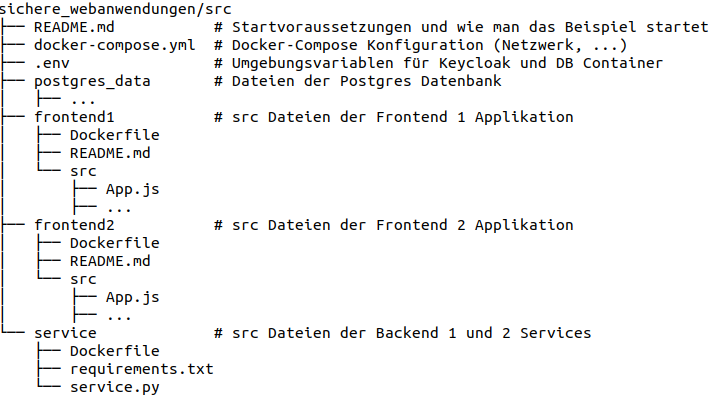
\includegraphics[width=1\textwidth]{Images/EbertScherer/srcDirectoryStructure.PNG}
	\caption{Struktur des Git-Verzeichnisses}
	\label{fig:EB_Struktur des Git-Verzeichnisses}
\end{figure}

%TODO wir müssen das Repo mit abgeben und dann darauf verweisen, wie es einen absatz weiter unten steht
In Abbildung \ref{fig:EB_Struktur des Git-Verzeichnisses} ist die Struktur des src Ordners zu sehen, welcher die von uns erstellen Dateien dieser Beispielwebanwendung enthält. Dieser src Ordner ist Teil des Git Repositories, welches unter \cite{SSEB1} heruntergeladen werden kann ist. Dort ist in der Datei 'src/README.md' \cite{SSEB2} die Anleitung zum Installieren und Starten dieser Beispielwebanwendung, sowie die Anmeldeinformationen für die von uns erstelle VMWare VM, die Keycloak Admin Console und einen registrierten Beispielbenutzer der Webanwendung. In der VMWare VM ist, wie in der 'src/README.md' näher erläutert, dieses Repository bereits heruntergeladen und die erforderlichen Befehle zur Installation wurden bereits ausgeführt. In der VM kann die Beispielwebanwendung mit 'cd /home/user/sichere\_webanwendungen/src \&\& docker-compose up' gestartet werden.

Die \texttt{docker-compose.yml} Datei enthält die Konfiguration für Docker-Compose. In \texttt{.env} wird der Pfad zum \texttt{postgres\_data} Ordner gesetzt, sowie das Adminpasswort für Keycloak. Keycloak ist in dieser Beispielwebanwendung bereits konfiguriert. Zum Beispiel sind Frontend 1 und 2 bereits in Keycloak als Clients eingetragen. 

Diese Konfiguration ist in der Datenbank bzw. dem \texttt{postgres\_data} Ordner gespeichert. Die Ordner \texttt{frontend1} und \texttt{frontend2} enthalten den Source Code für die Frontend Applikationen. Die zwei Frontend Applikationen sind außer verschiedener Farben im HTML identisch. Backend 1 und 2 sind ebenfalls identisch. Ihr Source Code ist im Ordner \texttt{service} zu finden.

Für Keycloak und die Datenbank waren bereits Docker Container Images vorhanden. Für die Frontend und Backend Komponenten haben wir neue Docker Container Images erstellt. Diese haben wir im Dockerhub unter \cite{EB42} hochgeladen. Das Dockerfile zum Bauen des jeweiligen Image ist im Source Folder der jeweiligen Komponente. Die Images können, müssen aber nicht lokal gebaut werden. Mit Docker-Compose werden diese automatisch von Dockerhub heruntergeladen. Die Anleitung zum lokalen Bauen der Container Images ist ebenfalls in der src/README.md Datei des Repositories \cite{SSEB2}.

Im src Ordner des geklonten Git Repositories \cite{SSEB1} kann der Befehl \texttt{docker-compose up} ausgeführt werden, um alle Container zu starten. Nach circa einer Minute ist Frontend 1 im Browser unter \texttt{localhost:3000} und Frontend 2 unter \texttt{localhost:3001} erreichbar. Im Folgenden wird eine Übersicht der Implementierung und Konfiguration der Komponenten und Flows gezeigt, sowie näher erläutert. Die genaue Dokumentation zur Implementierung des Systems kann im Code, z.B. im Git Repository \cite{SSEB1} oder in der VM, über DocStrings, Kommentaren und einer Dokumentation nachgelesen werden.


\subsection{Keycloak} \label{EB_Keycloak}

Der Keycloak Authorization Server ist unter \texttt{localhost:8080} erreichbar. Die Security Admin Console ist eine GUI zum Konfigurieren von Keycloak für Keycloak Administratoren. Über die URL  \texttt{localhost:8080/auth/admin/} ist diese GUI erreichbar. Im Beispiel kann man sich dort mit dem Benutzernamen \texttt{admin} und Passwort \texttt{iuq123} anmelden. Als Alternative zur GUI kann Keycloak auch über die sogenannte Admin CLI konfiguriert werden.

\subsubsection{Realms}\label{EB_Realms}

Keycloak hat ein Konzept namens \textit{Realms}. Jeder Realm hat eine Menge von Clients und Benutzern. Ein Realm ist wie eine Sandbox. Die Clients und Benutzer eines Realms sind isoliert von Clients und Benutzern anderer Realms \cite[Core Concepts and Terms]{SSEB_keycloakDocs}.

Beim ersten Start von Keycloak erstellt Keycloak einen vordefinierten Realm. Dieser wird \textit{master} Realm genannt. Der \textit{master} Realm enthält unter anderem den Keycloak Administrator-Benutzer. Außerdem fügt Keycloak die Security Admin Console und Admin CLI automatisch als Clients dem \textit{master} Realm hinzu. Aus Sicherheitsgründen sollten weitere Benutzer und Clients in einem neuen Realm konfiguriert werden, damit versehentliche Änderungen der Realmeinstellungen weniger schwerwiegend sind \cite[Master Realm]{SSEB_keycloakDocs}. Es können auch weitere Administrator-Benutzer für Realms erstellt werden. Administrator-Benutzer im Master Realm haben Zugriff auf alle Realms,  Administrator-Benutzer in anderen Realms haben nur Zugriff auf ihren eigenen Realm \cite[Master Realm]{SSEB_keycloakDocs}.

Für das Beispiel wurde ein neuer Realm mit dem Namen \texttt{Test} erstellt. In der Security Admin Console ist der Test Realm standardmäßig ausgewählt. Dort kann in der linken Navigationsleiste unter \textit{Realm Settings} der ausgewählte Realm konfiguriert werden. Zum Beispiel kann dort im Tokens Tab die Verfallszeit des Access Tokens gesetzt werden. Weiter kann im Login Tab eingestellt werden, dass alle Anfragen an Keycloak über TLS verschlüsselt werden müssen.

\subsubsection{Clients}

In der linken Navigationsleiste der Security Admin Console können unter \textit{Clients} alle Clients des Realms angezeigt werden und neue Clients erstellt werden. Im Beispiel wurden die folgenden vier Clients erstellt: \texttt{frontend1, frontend2, service1, service2}. Die Konfiguration der Clients kann unter \texttt{Edit} angezeigt werden.

\begin{figure}[!ht]
	\centering
	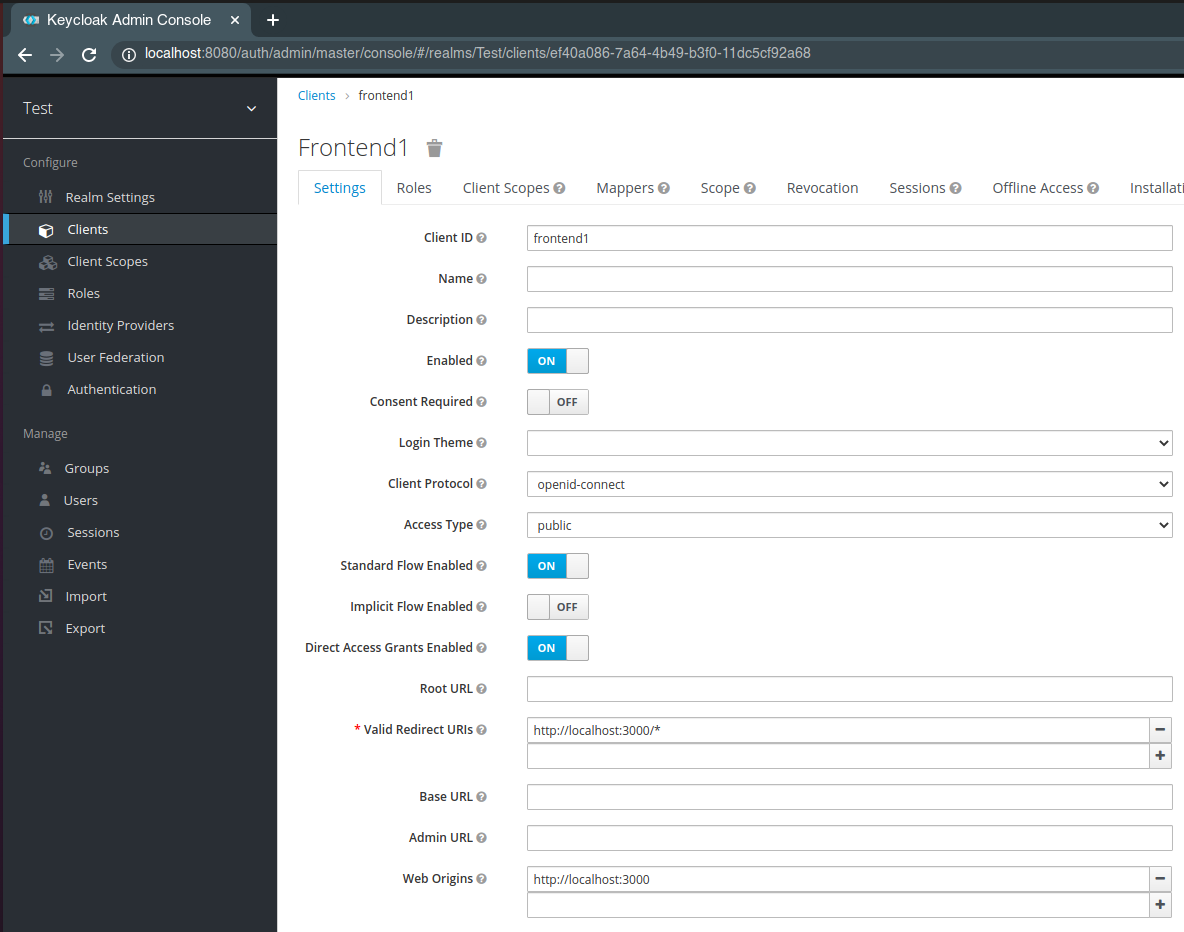
\includegraphics[width=1\textwidth]{Images/EbertScherer/KeycloakClientConfig.PNG}
	\caption{Keycloak \texttt{frontend1} Client Konfiguration}
	\label{fig:EB_Keycloak frontend1 Client Konfiguration}
\end{figure}

In Abbildung \ref{fig:EB_Keycloak frontend1 Client Konfiguration} ist die Konfiguration des \texttt{frontend1}-Clients gezeigt. Die folgende Auflistung beschreibt wichtige Felder in Abbildung \ref{fig:EB_Keycloak frontend1 Client Konfiguration}:
\begin{itemize}
	\item \emph{Client ID:} \texttt{frontend1} ist die Client ID für Frontend 1.
	
	\item \emph{Consent Required:} Setzt fest, ob der Benutzer den von Clients gewünschten Scopes zustimmen muss. Das ist der im Authorization Code Flow in Sektion \ref{EB_Authentifizierung_eines_Benutzers} beschriebene Schritt 4.
	
	\item \emph{Client Protocol:} Legt das Protokoll OIDC fest, welches der Client bei der Kommunikation mit Keycloak verwendet.
	
	\item \emph{Access Type:} In Sektion \ref{EB_Client} wurden zwei Arten von Clients für Web SSO beschrieben. Der Wert \textit{public} ist für Clients der ersten Art, die Frontend Applikationen. Backend 1 und 2 haben die Client ID \texttt{service1} und \texttt{service2}. Diese sind Clients der zweiten Art. Bei diesen ist der Access Type auf \texttt{bearer-only} gesetzt. Dadurch können die Backend Services keinen Authorization Code Flow anstoßen.
	
	\item \emph{Valid Redirect URIs:} Hier können möglichst präzise Validierungsrichtlinien für Redirect URIs gesetzt werden, nach \ref{Registrierung_redirect_uri}.
	
	\item \emph{Web Origins:} Dadurch ist für den Client der HTTP Header \texttt{Access-Control-Allow-Origin: http://localhost:3000} in Nachrichten von Keycloak zum Client enthalten. Dieses Feld muss auf die URL des Frontends gesetzt werden, um CORS zu erlauben. Ansonsten akzeptiert der Browser eingehende Anfragen bzw. Redirects von Keycloak nicht.
\end{itemize}

\subsubsection{Client Scopes}

In der linken Navigationsleiste der Security Admin Console kann auf die Keycloak Client Scopes zugegriffen werden. Für ein Keycloak Client Scope können beliebig viele sogenannte \textit{Protocol Mapper} definiert werden. Mit Protocol Mappern können die Claims von z.B. dem ID- und Access Token und die zurückgegebenen Claims des UserInfo Endpunkts konfiguriert werden. Dazu gehört unter anderem das Hinzufügen weiterer Scopes im \texttt{scopes} Claim und weiterer Audiences im \texttt{aud} Claim des Access Tokens. Es können auch neue Claims erstellt werden, welche dem ID- oder Access Token hinzugefügt oder vom UserInfo Endpunkt zurückgegeben werden. Über Protocol Mapper können Benutzern auch Rollen für Role Based Access Control zugewiesen werden. Wie in der Abgrenzung in Sektion \ref{EB_Abgrenzung} erläutert, wird Role Based Access Control in dieser Arbeit jedoch nicht näher betrachtet. 

Im Folgenden werden zwei Beispiele für Keycloak Client Scopes gezeigt. Im ersten Beispiel werden die zwei Backend Clients mit Client ID \texttt{service1} und \texttt{service2} dem \texttt{aud} Claim des Access Tokens hinzugefügt. Unter \texttt{Client Scopes} und \texttt{Create} wird dafür, wie in Abbildung \ref{fig:EB_Keycloak Client Scope für Audience Claim} gezeigt, ein neuer Client Scope erstellt mit dem Namen \texttt{backend\_audience}. Ein wichtiges Feld in \ref{fig:EB_Keycloak Client Scope für Audience Claim} ist \texttt{Include In Token Scope}. Ist dieses Feld \texttt{ON}, dann ist der Name des Client Scopes im \texttt{scopes} Claim des Access Tokens enthalten. In diesem Fall ist das Feld \texttt{OFF}, da nur der \texttt{aud} Claim angepasst werden soll.

\begin{figure}[!ht]
	\centering
	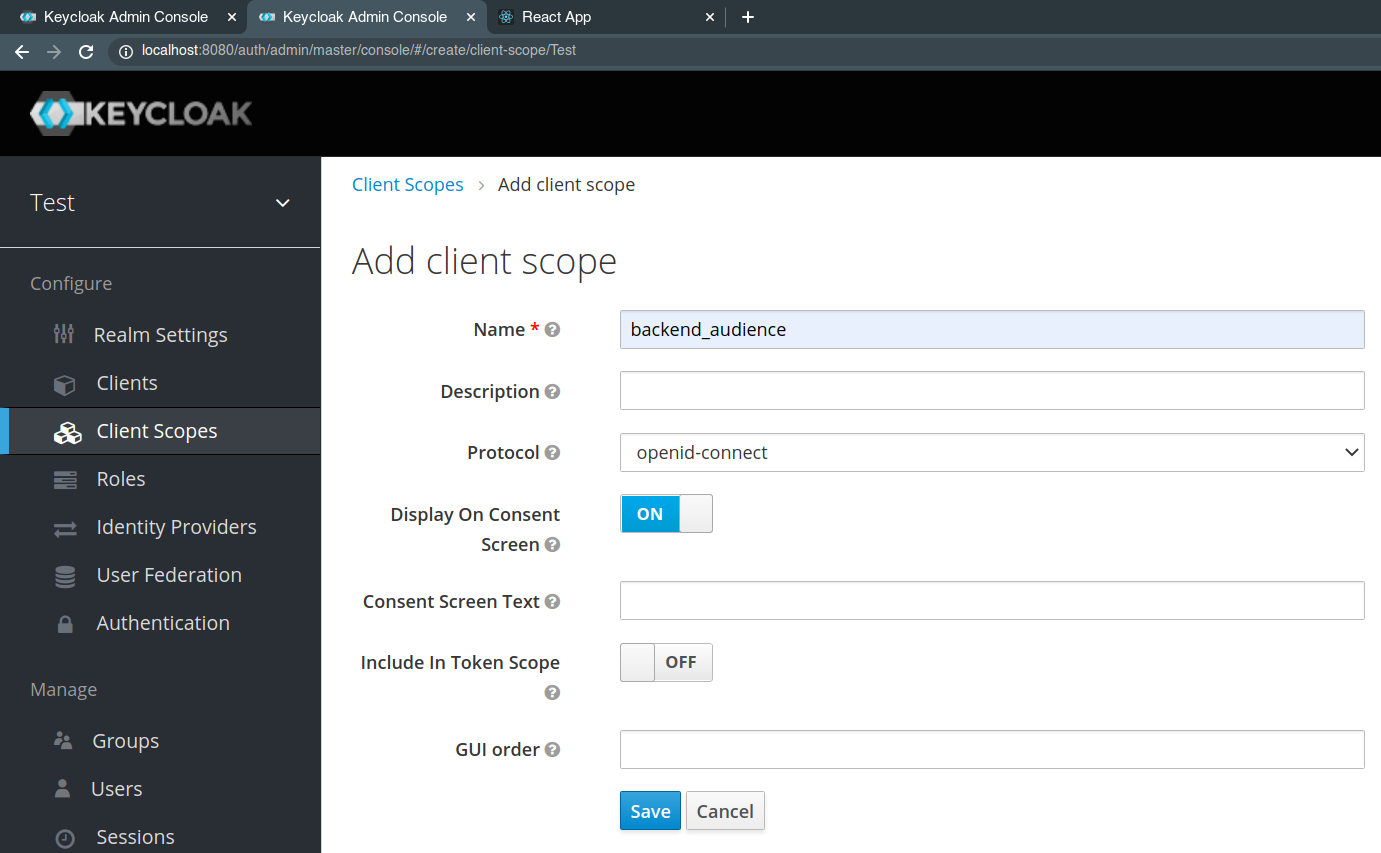
\includegraphics[width=1\textwidth]{Images/EbertScherer/KeycloakNewAudClientScope.PNG}
	\caption{Keycloak Client Scope für Audience Claims}
	\label{fig:EB_Keycloak Client Scope für Audience Claim}
\end{figure}

Für den Client Scope werden im \texttt{Mappers} Tab über \texttt{Create} zwei Protocol Mapper vom Typ \texttt{Audience} erstellt, jeweils einen Protocol Mapper für jeden Backend Client. Die Konfiguration für den ersten Backend Client wird in Abbildung \ref{fig:EB_Keycloak Protocol Mapper für Audience Claim} gezeigt. Im \texttt{Included Client Audience} Feld kann aus einer Liste aller Clients der Client ausgewählt werden, welcher dem \texttt{aud} Claim hinzugefügt werden soll. Für den zweiten Protocol Mapper ist an dieser Stelle der Client mit der ID \texttt{service2} eingetragen. Über die \texttt{Add to ID token} und \texttt{Add to access token} Felder wird festgelegt, dass die Änderung nur beim \texttt{aud} Claim des Access Tokens stattfinden soll.

\begin{figure}[!ht]
	\centering
	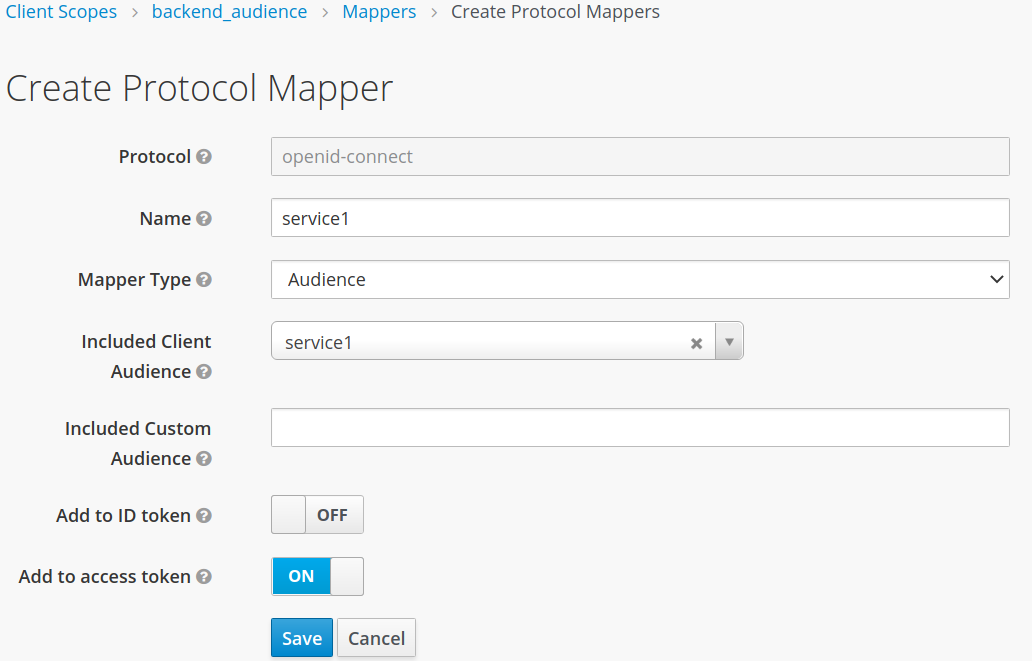
\includegraphics[width=1\textwidth]{Images/EbertScherer/KeycloakNewAudProtocolMapper.PNG}
	\caption{Keycloak Protocol Mapper für Audience Claims}
	\label{fig:EB_Keycloak Protocol Mapper für Audience Claim}
\end{figure}

Abschließend kann der Client Scope einem oder mehreren Clients hinzugefügt werden. Die im Client Scope definierten Änderungen werden bei den ausgewählten Clients angewandt. In diesem Beispiel sollen die \texttt{aud} Claims der Access Tokens an die zwei Frontend Applikationen angepasst werden. In Abbildung \ref{fig:EB_Keycloak Client Scope einem Client zuweisen} wird das Hinzufügen des \texttt{backend\_audience} Client Scopes zum \texttt{frontend1} Client gezeigt. Im \texttt{Client Scopes} Tab des \texttt{frontend1} Clients wird dazu der \texttt{backend\_audience} Client Scope ausgewählt. Dieser kann dann mit \textit{Add selected} der Liste der zugewiesenen Standard Client Scopes für den Client hinzugefügt werden.

\begin{figure}[!ht]
	\centering
	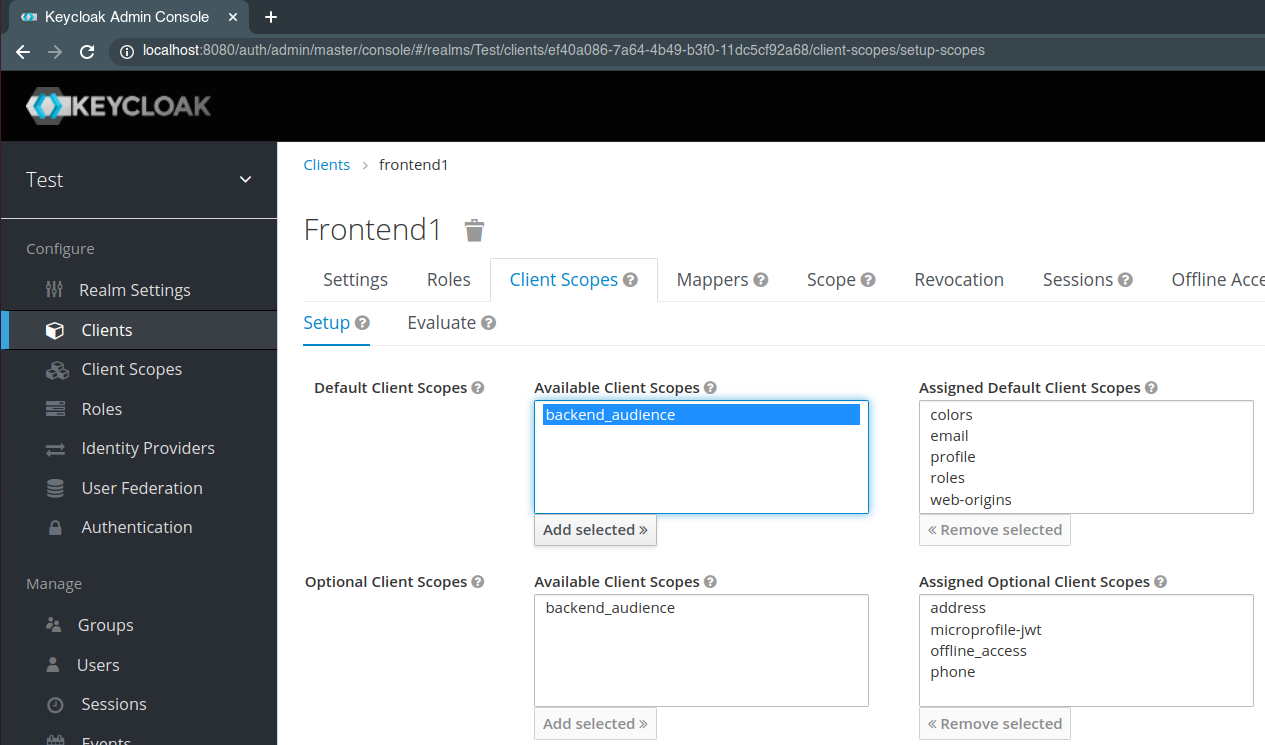
\includegraphics[width=1\textwidth]{Images/EbertScherer/KeycloakAddAudClientScope.PNG}
	\caption{Zuweisung eines Keycloak Client Scopes zu einem Client}
	\label{fig:EB_Keycloak Client Scope einem Client zuweisen}
\end{figure}

Im zweiten Beispiel soll ein neuer Claim \texttt{GUI\_Color} erstellt werden. Dieser Claim soll im ID Token enthalten sein und vom UserInfo Endpunkt zurückgegeben werden. Die \texttt{GUI\_Color} soll nicht bei allen Benutzern gleich sein, sondern sie soll der Lieblingsfarbe des Benutzers entsprechen.

In Keycloak können Benutzer Attribute haben. Attribute sind Key-Value Paare. Diese können z.B. in der Security Admin Console, der Admin CLI oder beim Registrieren des Benutzers gesetzt werden. In Abbildung \ref{fig:EB_Keycloak Client User Attribut} wurde in der linken Navigationsleiste unter \texttt{Users} das \texttt{Attributes} Tab des \texttt{admin} Benutzers ausgewählt und das Attribut \texttt{favorite\_color} mit dem Value \texttt{blue} hinzugefügt. Dieses Attribut kann über einen Protocol Mapper referenziert werden.

\begin{figure}[!ht]
	\centering
	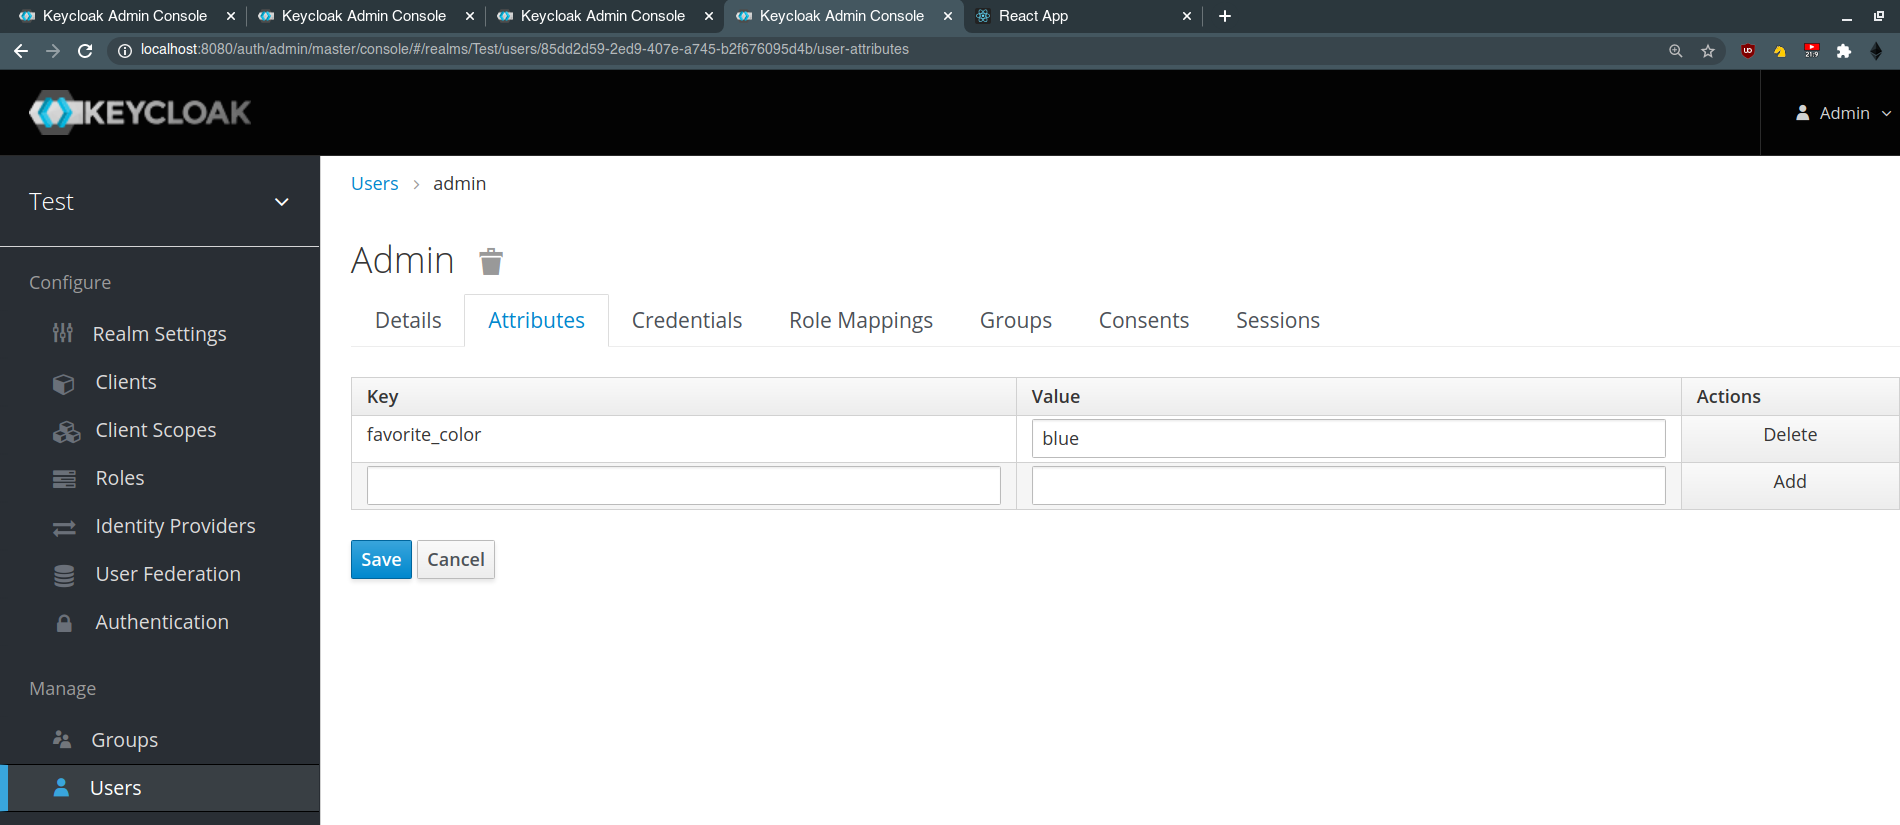
\includegraphics[width=1\textwidth]{Images/EbertScherer/KeycloakNewUserAttribute.PNG}
	\caption{Keycloak Client Benutzer Attribut}
	\label{fig:EB_Keycloak Client User Attribut}
\end{figure}

Davor wird ein neuer Client Scope erzeugt. Die Konfiguration dieses Client Scopes ist in Abbildung \ref{fig:EB_Keycloak Client Scope für User Attribut} gezeigt. Anders als im ersten Beispiel ist \texttt{Include In Token Scope} auf \texttt{ON}, damit der Name des Client Scopes \texttt{colors} im \texttt{scopes} Claim des Access Tokens enthalten ist.

\begin{figure}[!ht]
	\centering
	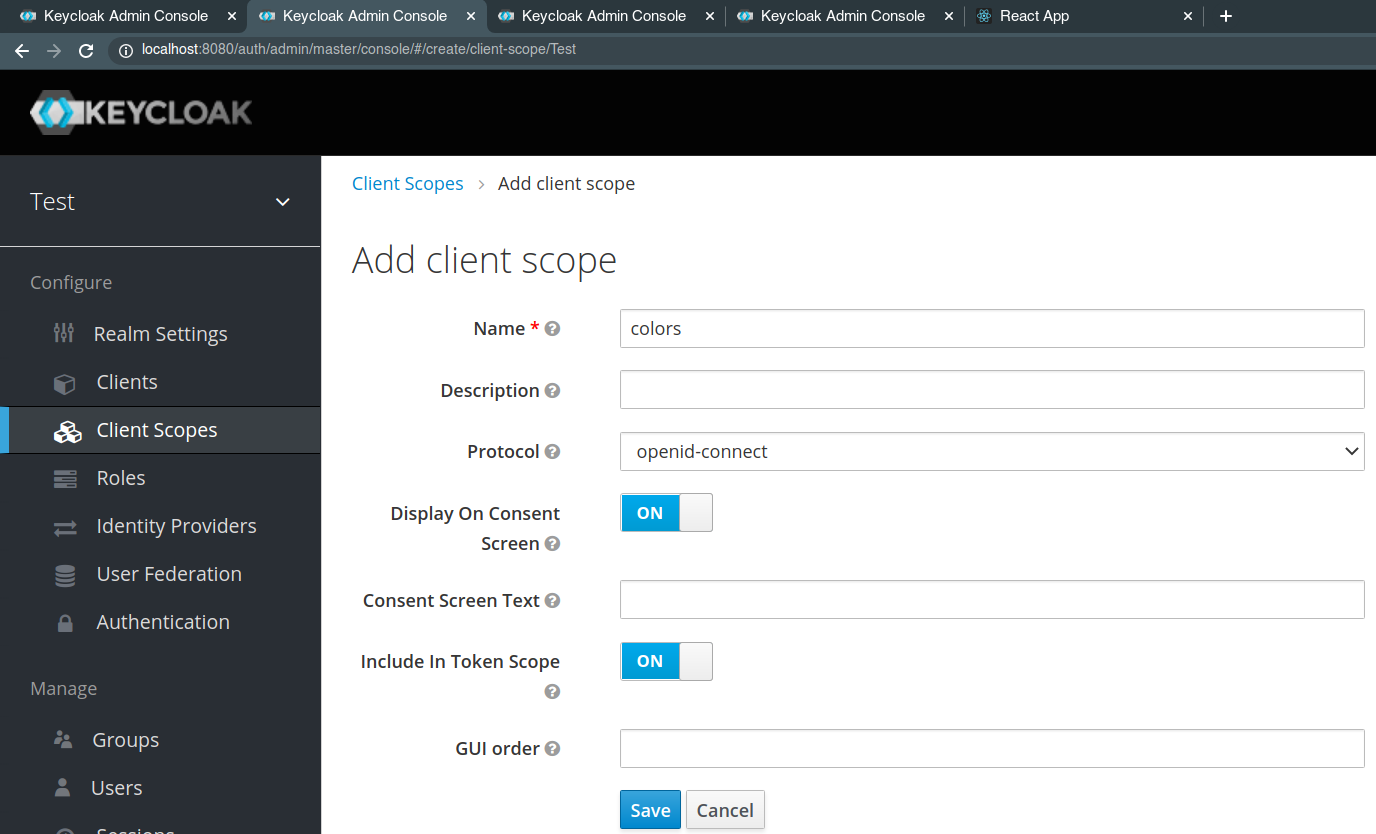
\includegraphics[width=1\textwidth]{Images/EbertScherer/KeycloakNewUserAttributeClientScope.PNG}
	\caption{Keycloak Client Scope für ein Benutzer Attribut}
	\label{fig:EB_Keycloak Client Scope für User Attribut}
\end{figure}

Danach wird diesem Client Scope der in Abbildung \ref{fig:EB_Keycloak Protocol Mapper fuer GUI color Claim} gezeigte Protocol Mapper hinzugefügt. Als \textit{Mapper Type} wird in diesem Fall \texttt{User Attribute} ausgewählt. Das \textit{User Attribute} Feld enthält den Namen des für den Benutzer angelegten Attributs. \textit{Token Claim Name} setzt den Key des Claims auf \texttt{GUI\_color}. \texttt{Add to ID token} und \texttt{Add to userinfo} ist beides auf \texttt{ON}, damit der Claim sowohl im ID Token enthalten ist als auch vom UserInfo Endpunkt zurückgegeben werden kann. Der Value dieses Claims ist dann der Wert des \texttt{favourite\_color} Attributes des authentifizierten Benutzers. Wenn für einen Benutzer kein \texttt{favourite\_color} Attribut hinzugefügt ist, dann ist der Claim nicht im ID Token und nicht in Antworten des UserInfo Endpunkts enthalten. Wie im ersten Beispiel muss der Client Scope den zwei Fontend Clients hinzugefügt werden.

\begin{figure}[!ht]
	\centering
	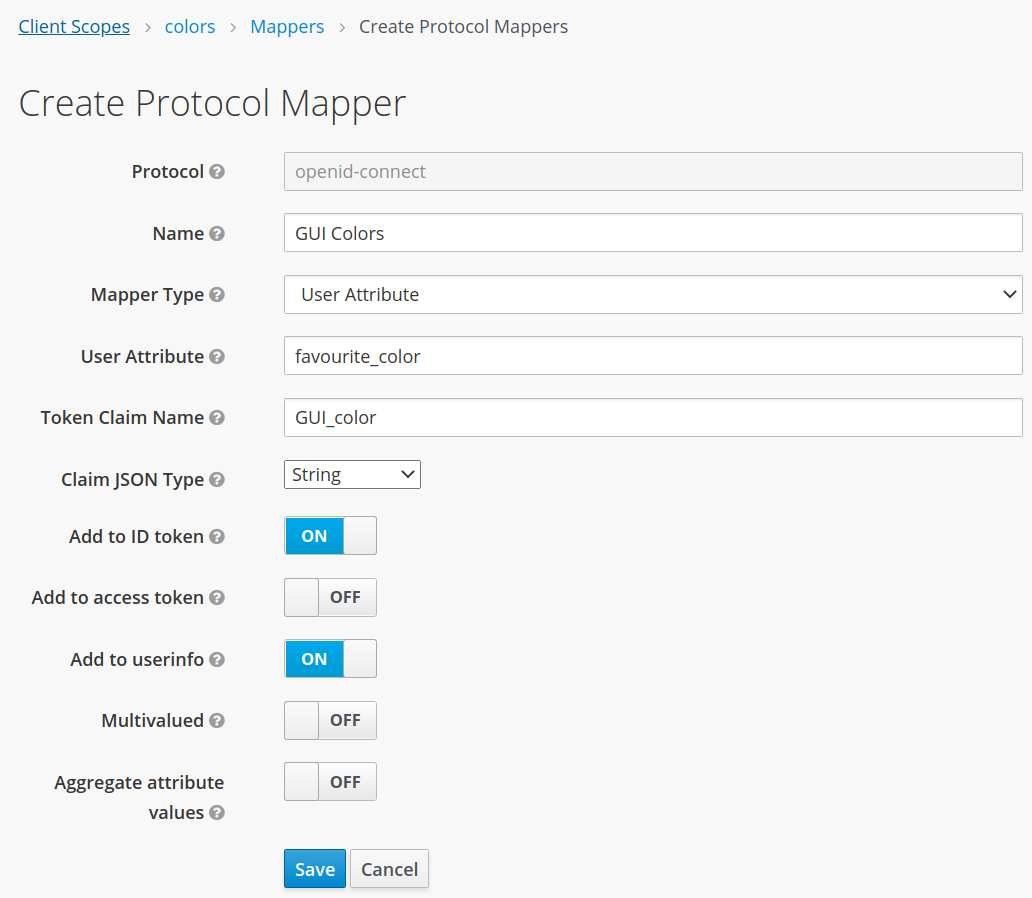
\includegraphics[width=1\textwidth]{Images/EbertScherer/KeycloakNewClaimProtocolMapper.PNG}
	\caption{Keycloak Protocol Mapper für \texttt{GUI\_color} Claim}
	\label{fig:EB_Keycloak Protocol Mapper fuer GUI color Claim}
\end{figure}



\subsection{Frontend}

Das Frontend verwendet das Web Framework \textit{ReactJS} \cite{EB43}. Für Keycloak gibt es sogenannte Adapter. Diese Adapter sind für verschiedenen Programmiersprachen und Systeme wie ReactJS verfügbar. Im Frontend wird der Adapter mit dem Namen \texttt{react-keycloak} verwendet \cite{EB36}. Ein Adapter ist mehr als eine Programmbibliothek oder ein Paket \cite{EB43}. Die Adapter sind eng in das System, wie ReactJS, integriert \cite{EB43}. Zum Beispiel implementiert der Adapter den Authorization Code Flow zur Authentifizierung eines Benutzers. Authentifiziert sich der Benutzer das erste Mal, dann kann dieser Flow mit dem Aufruf der \texttt{login()} Funktion initiiert werden. Wenn sich der Benutzer bereits bei einem anderen Client authentifiziert hat, führt der Adapter den Authorization Code Flow beim Aufrufen der Website im Hintergrund aus, um den Benutzer ohne erneute Eingabe von Anmeldeinformationen wie Benutzernamen und Passwort zu authentifizieren. Im nachfolgenden Beispiel wird das anhand von Screenshots der Anwendung noch einmal ausführlicher beschrieben.

In \ref{fig:EB_Nicht Authentifiziert} ist eine Abbildung der Website von \texttt{frontend1} zu sehen. Dabei hat sich der Benutzer noch nicht authentifiziert. Über die \texttt{GET SERVICE 1 DATA} und \texttt{GET SERVICE 2 DATA} Buttons wird jeweils eine Funktion aufgerufen, welche eine HTTP Post Anfrage an den jeweiligen Backend Service, die Clients mit ID \texttt{service1} und \texttt{service2}, sendet. Ist ein Benutzer authentifiziert, dann wird der Access Token im Bearer Header der Anfrage mitgesendet. Die Backend Services überprüfen, ob eingehende Nachrichten einen validen Access Token enthalten. Bei Erfolg liefern diese die Identifikationsnummer für den Benutzer, den \texttt{sub} Claim, mit dem HTTP-Statuscode \texttt{200} zurück. Andernfalls wird, wie in Abbildung \ref{fig:EB_Nicht Authentifizierte Anfrage an Backend} gezeigt, \texttt{FAILED} mit Statuscode \texttt{402} zurückgegeben und angezeigt. Der Backend Service wird in der nächsten Sektion \ref{EB_Backend} näher erläutert.

\begin{figure}[!ht]
	\centering
	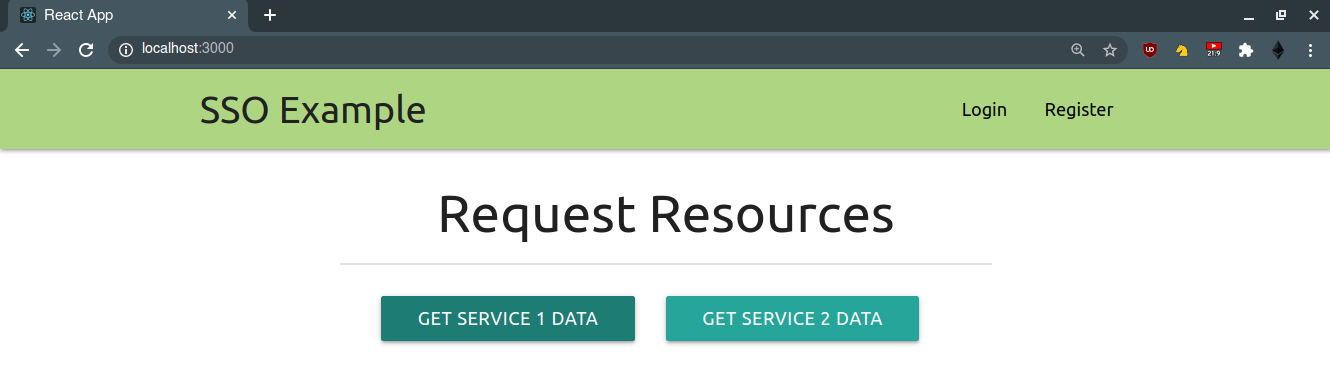
\includegraphics[width=1\textwidth]{Images/EbertScherer/FrontendLoggedOut.PNG}
	\caption{Frontend Client GUI - Nicht Authentifiziert}
	\label{fig:EB_Nicht Authentifiziert}
\end{figure}

\begin{figure}[!ht]
	\centering
	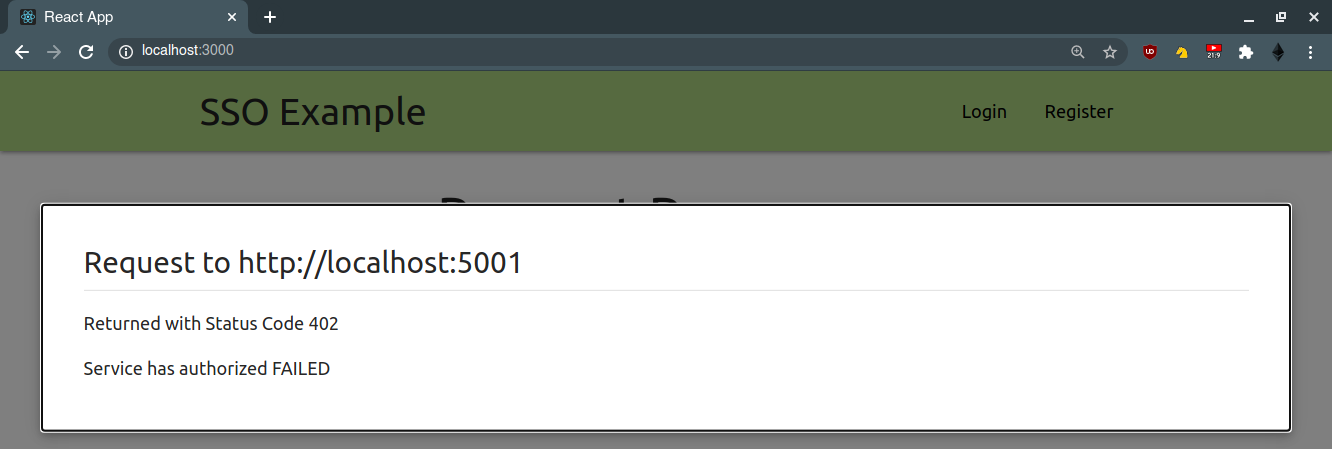
\includegraphics[width=1\textwidth]{Images/EbertScherer/FrontendLoggedOutBackendRequest.PNG}
	\caption{Frontend Client GUI - Nicht Authentifizierte Anfrage an Backend}
	\label{fig:EB_Nicht Authentifizierte Anfrage an Backend}
\end{figure}

In der oberen Navigationsleiste sind auf der rechten Seite zwei Buttons, über die sich Benutzer authentifizieren oder registrieren können. Für beides bietet der Keycloak Adapter Funktionen an, welche beim Klicken des jeweiligen Buttons ausgeführt werden. Beim Klicken des \texttt{Login} Buttons wird der Authorization Code Flow initiiert. Der Benutzer wird dann zu Keycloaks Authorization Endpunkt geleitet. Das ist in Abbildung \ref{fig:EB_Login Form des Authorization Endpunkts} dargestellt. In der Adresszeile sieht man die Addresse des Authorization Endpunkts und einen Teil des Query-Strings, der die Parameter des Authorization Requests enthält. Der Benutzer kann sich hier z.B. als Admin Benutzer mit 'admin:iuq123' (Username:Password), oder mit dem bereits registrierten Beispielbenutzer 'user:user' einloggen. Für beide Benuter sind unterschiedliche Lieblingsfarben als Attribute konfiguriert.

\begin{figure}[!ht]
	\centering
	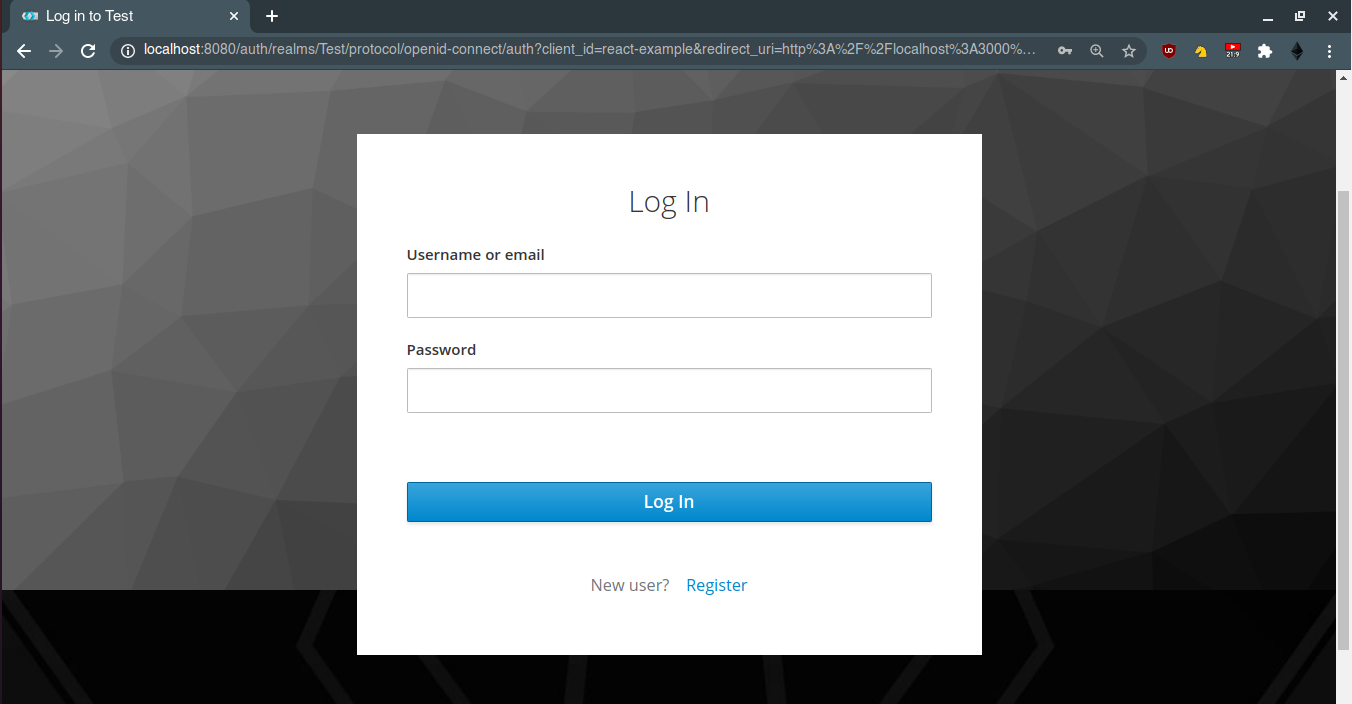
\includegraphics[width=1\textwidth]{Images/EbertScherer/FrontendLoginForm.PNG}
	\caption{Keycloak GUI - Login Form des Authorization Endpunkts}
	\label{fig:EB_Login Form des Authorization Endpunkts}
\end{figure}

Nach einer erfolgreichen Authentifizierung mit dem Authorization Code Flow wird der Benutzer zurück auf die Website des Frontend Clients geleitet. Anfragen an den Backend Service sind nun erfolgreich. Das ist in Abbildung \ref{fig:EB_Authentifizierte Anfrage an Backend} dargestellt. Access Tokens werden automatisch im Hintergrund erneuert. Dabei sendet der Adapter Anfragen mit dem Refresh Token an Keycloaks Token Endpunkt. Standardmäßig hat der Refresh Token in Keycloak eine Verfallszeit von 10 Stunden. Über den Token Endpunkt ruft der Adapter ebenfalls automatisch neue Refresh und ID Token ab.

\begin{figure}[!ht]
	\centering
	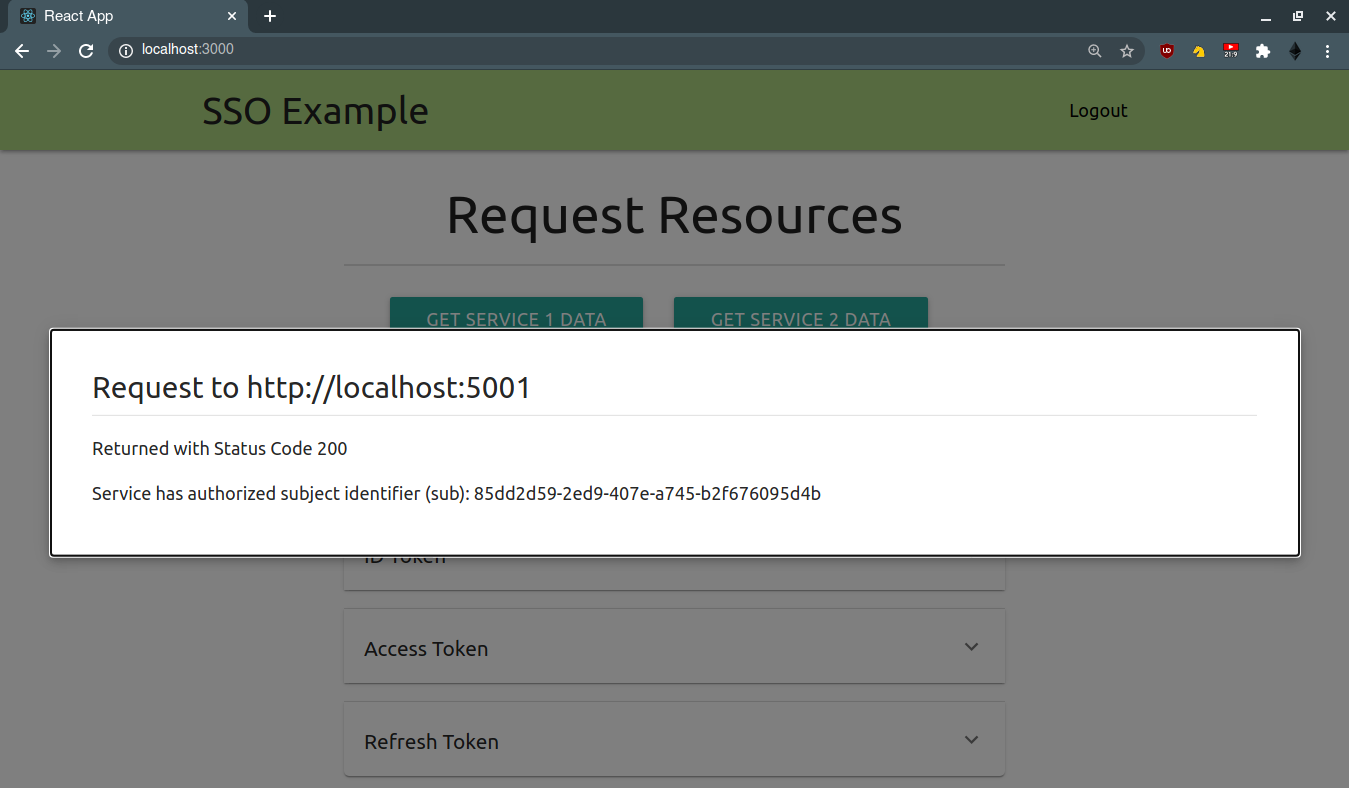
\includegraphics[width=1\textwidth]{Images/EbertScherer/FrontendLoggedInBackendRequest.PNG}
	\caption{Frontend Client GUI - Authentifizierte Anfrage an Backend}
	\label{fig:EB_Authentifizierte Anfrage an Backend}
\end{figure} 

Der Adapter stellt außerdem APIs zum Abrufen von Tokens zur Verfügung. Ist ein Benutzer authentifiziert, dann werden ID-, Access-, und Refresh Token in der GUI dekodiert angezeigt. Abbildung \ref{fig:EB_Token} zeigt davon einen Ausschnitt.

\begin{figure}[!ht]
	\centering
	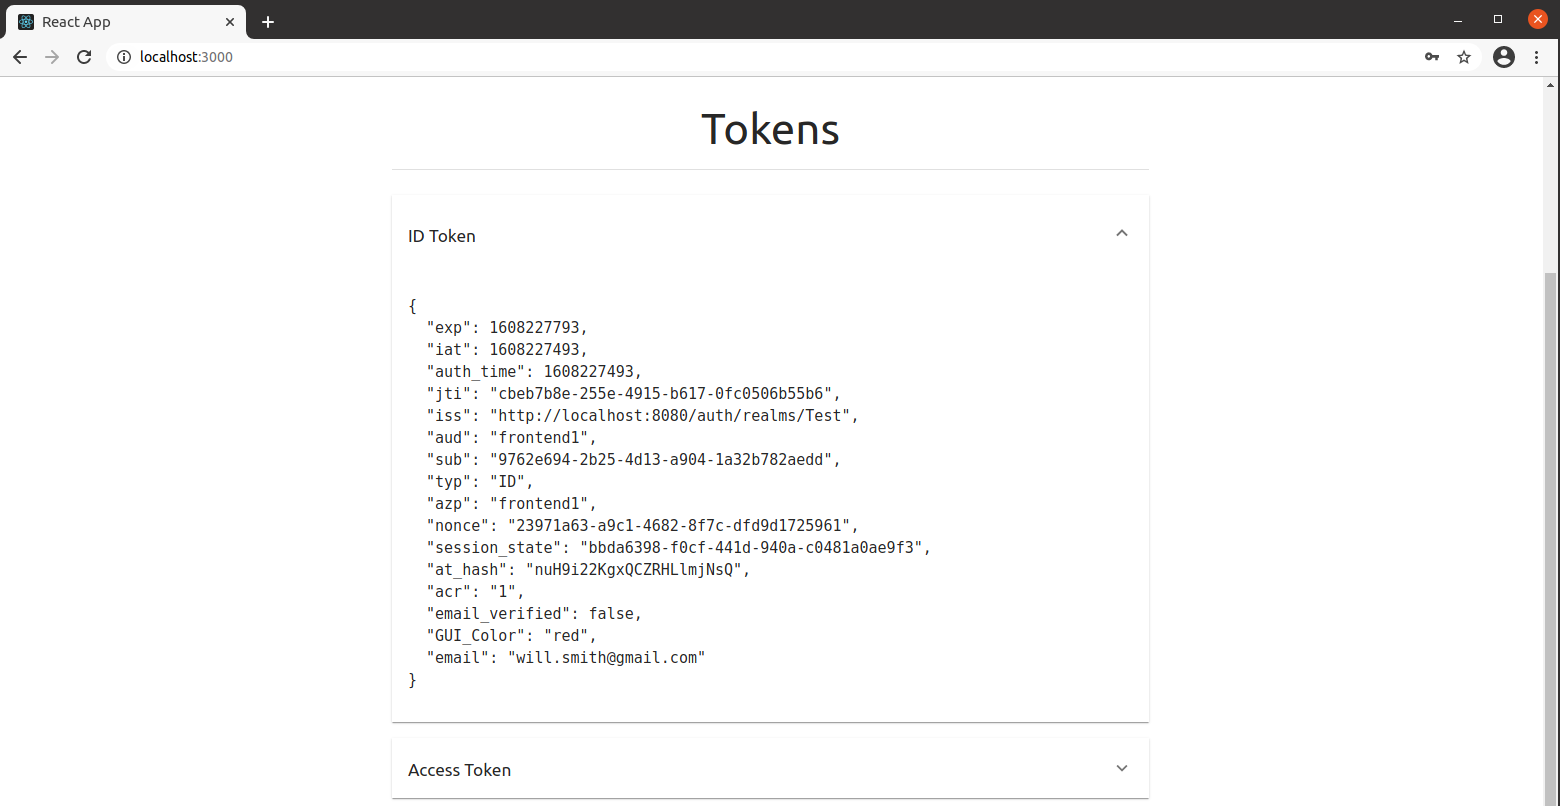
\includegraphics[width=1\textwidth]{Images/EbertScherer/FrontendIDTokenExample.PNG}
	\caption{Frontend Client GUI - Token}
	\label{fig:EB_Token}
\end{figure}

Durch die erfolgreichen Authentifizierung mit dem Authorization Code Flow hat Keycloak den in Sektion \ref{EB_Authentifizierung_eines_Benutzers} beschriebenen \texttt{KEYCLOAK\_IDENTITY} Cookie für Keycloaks Authorization Endpunkt gesetzt. Dieser Cookie enthält einen ID Token. In Abbildung \ref{fig:EB_ID Token Cookie für Keycloak} ist manuell zum Authorization Endpunkt navigiert worden und über die Chrome Developer Console kann der Cookie angezeigt werden. Durch diesen Cookie wird, wie in Abbildung \ref{fig:EB_Snapshot nach Aufruf des zweiten Frontends} gezeigt, der Benutzer beim Aufruf des zweiten Frontend Clients automatisch authentisiert.

\begin{figure}[!ht]
	\centering
	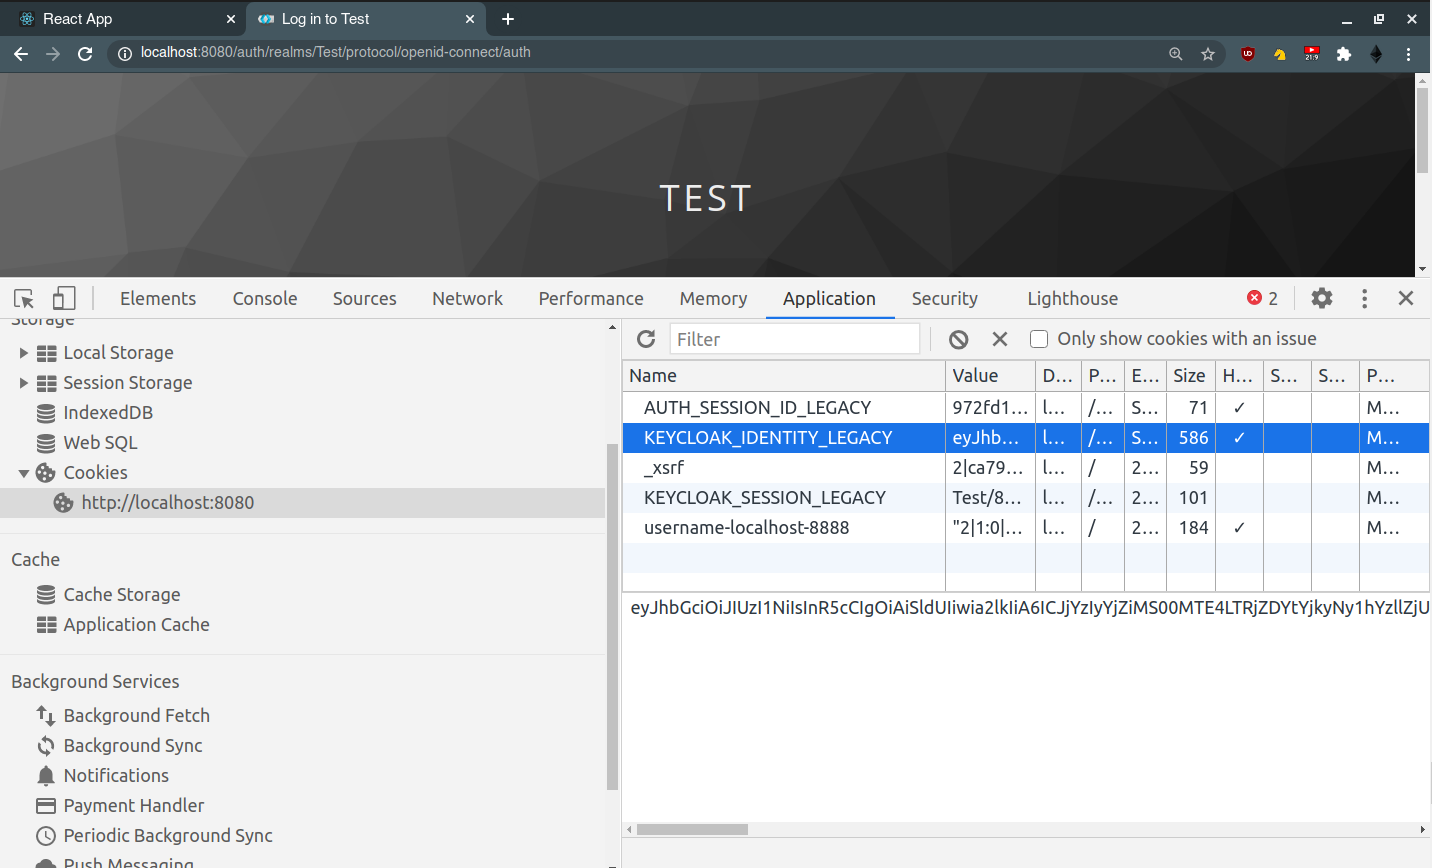
\includegraphics[width=1\textwidth]{Images/EbertScherer/FrontendCookieForKeycloak.PNG}
	\caption{ID Token Cookie für Keycloak}
	\label{fig:EB_ID Token Cookie für Keycloak}
\end{figure}

\begin{figure}[!ht]
	\centering
	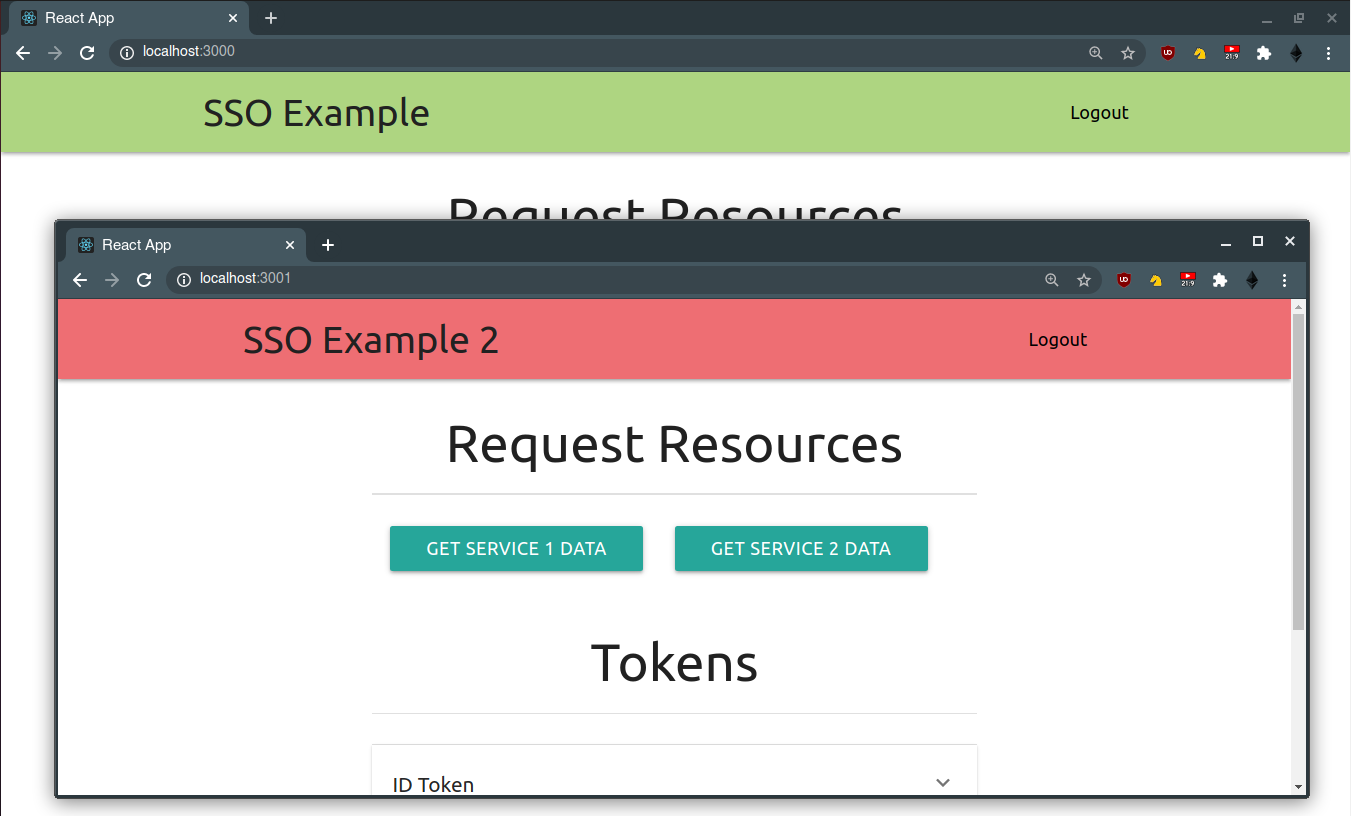
\includegraphics[width=1\textwidth]{Images/EbertScherer/FrontendOpenSecondFrontend.PNG}
	\caption{Snapshot nach Aufruf des zweiten Frontends}
	\label{fig:EB_Snapshot nach Aufruf des zweiten Frontends}
\end{figure}


\subsection{Backend} \label{EB_Backend}

Die zwei Backend Services lauschen auf verschiedenen Ports, sind aber im Hinblick auf die Funktionsweise gleich. Sie sind in Python geschrieben und verwenden das Web MicroFramework \textit{Flask} \cite{EB48}. \texttt{Flask-CORS}, eine Erweiterung von Flask, wird verwendet, um CORS für die Sender aller eingehenden Anfragen zu erlauben \cite{EB49}. \texttt{PyJWT} implementiert den JSON Web Token (JWT) Standard (RFC 7519 \cite{SSEB_RFC7519}) \cite{EB51}. Das Backend verwendet PyJWT um Access Tokens zu decodieren.

Eingehende Anfragen werden in zwei Schritten abgearbeitet. Im ersten Schritt wird der Access bzw. Bearer Token aus dem HTTP Authorization Header extrahiert. Schlägt dies fehl, z.B. wenn die Anfrage keinen HTTP Authorization Header enthält, dann wird der Text \texttt{FAILED} im HTTP Message Body mit Statuscode \texttt{402} zurückgegeben. Andernfalls wird der extrahierte Token an die in der folgenden Auflistung gezeigten Funktion übergeben.

\begin{lstlisting}[caption=Token Validierung im Backend, captionpos=b, language=python, label=validateTokenFunction]
def validate_token(token):
  # Decode Access Token without validating it.
  try:
    decoded_token = jwt.decode(token, verify=False)
  except Exception:
    return 'FAILED', 402
  # Invalid if this client's ID is not in 'aud' claim
  if 'aud' not in decoded_token:
    return 'FAILED: no "aud" claim in token', 402
  if client_ID not in decoded_token['aud']:
    return f'FAILED: {client_ID} not in "aud" claim', 402
  # Online Signatur Validation
  url = (f'http://{KEYCLOAK_HOST}/auth/realms/{REALM_NAME}' +
          '/protocol/openid-connect/userinfo')
  headers = {"Authorization": f'Bearer {token}'}
  r = requests.get(url, headers=headers)
  if r.status_code != 200:
    return 'Invalid signature', 402
  r_json = json.loads(r.text)
  return f'subject identifier (sub): {r_json["sub"]}', 200
\end{lstlisting}

Dabei wird der Token als erstes über die PyJWT Bibliothek dekodiert. Die Signatur des Tokens wird dort noch nicht validiert. Danach wird überprüft, ob der Token einen \texttt{aud} Claim enthält und ob die ID des jeweiligen Backend Clients im \texttt{aud} Claim enthalten ist. Die Motivation für diese Art der Überprüfung wurde in Sektion \ref{EB_Zugriff auf geschützte Ressourcen} erläutert. Für die Validierung der Signatur wird die in Sektion \ref{EB_Validieren des Access Tokens} beschriebene Online Validierung eingesetzt, bei der der Token über Keycloak validiert wird. Dabei wird eine Anfrage an Keycloaks UserInfo Endpunkt mit dem Token im HTTP Authorization Header als Bearer Token gesendet. Bei valider Signatur liefert die Keycloak Anfrage den Statuscode \texttt{200} und die für den UserInfo Endpunkt und den Access Token zugelassenen Claims im HTTP Message Body zurück. 

Die Funktion \ref{validateTokenFunction} gibt einen Tuple mit zwei Elementen zurück und implementiert die zuvor beschriebene Vorgehensweise. Das erste Element wird als HTTP Message Body und das zweite Element als Statuscode an den Sender der Anfrage an das Backend zurückgesendet. Bei nicht erfolgreicher Validierung des Tokens wird der Statuscode \texttt{402} mit Fehlermeldung im HTTP Message Body zurückgegeben. Andernfalls wird die ID des Benutzers des Access Tokens und Statuscode \texttt{200} zurückgegeben.


\section{Zusammenfassung}

In dieser Arbeit ist SSO bei Webanwendungen vorgestellt worden. Dabei wurde speziell das OIDC Protokoll und Keycloak, sowie die Sicherheit dieser analysiert. Keycloak unterstützt OIDC und implementiert geeignete Gegenmaßnahmen, um sich und Keycloaks Benutzer vor den unter anderem in Sektion \ref{SSEB_Threat Model} Threat Model vorgestellten möglichen Threats bei Web SSO zu schützen. Aus diesem Grund kann Keycloak und dessen Adapter, wie in der implementierten und in Sektion \ref{EB_Beispielwebanwendung} vorgestellten Beispielwebanwendung verwendet werden, um Web SSO sicher zu implementieren.


